\newcommand{\anonsection}[1]{\section*{#1}\addcontentsline{toc}{section}{#1}}
\newcommand{\anonsubsection}[1]{\subsection*{#1}\addcontentsline{toc}{subsection}{#1}}
\newcommand{\anonsubsubsection}[1]{\subsubsection*{#1}\addcontentsline{toc}{subsubsection}{#1}}

\documentclass[11pt]{article}

\usepackage[T2A]{fontenc}
\usepackage[utf8]{inputenc}
\usepackage[russian]{babel}

\usepackage{indentfirst}
\usepackage{geometry}
\usepackage{graphicx}
\usepackage{caption}
\usepackage{subcaption}
\usepackage{mathtools}

\usepackage{amsmath, amssymb, amsfonts, amsthm}

\newtheorem{theorem}{Теорема}
\newtheorem{definition}{Определение} 
\newtheorem{statement}{Утверждение}
\newtheorem{property}{Свойство}

\DeclareMathOperator{\Uni}{\mathbb{U}}
\DeclareMathOperator{\Ind}{\mathbb{I}}
\DeclareMathOperator{\Bin}{\mathrm{Bin}}
\DeclareMathOperator{\Bern}{\mathrm{Bern}}
\DeclareMathOperator{\Geom}{\mathrm{Geom}}
\DeclareMathOperator{\Norm}{\mathrm{N}}
\DeclareMathOperator{\Expon}{\mathrm{Exp}}
\DeclareMathOperator{\Pois}{\mathrm{Pois}}
\DeclareMathOperator{\Exp}{\mathbb{E}}
\DeclareMathOperator{\esssup}{\text{esssup}}

\geometry{a4paper}
\sloppy

\begin{document}

\begin{titlepage}
    \begin{centering}
        
\includegraphics[width=0.5\textwidth]{resources/msu.png}\\
        {\scshape Московский государственный университет имени М.~В.~Ломоносова}\\
        Факультет вычислительной математики и кибернетики\\
        Кафедра системного анализа\\
        \vfill
        {\LARGE Отчет по компьютерному практикуму к курсу}\\
        \vspace{1cm}
        {\Huge\bfseries "<Стохастический анализ и моделирование">\\}
    \end{centering}
    \vspace{1cm}
    \begin{flushright}
        \begin{large}
            {\itshape Студент 415 группы\\}
            Е.~В.~Гуров\\
            \vspace{5mm}
            {\itshape Руководитель практикума\\}
            к.ф.-м.н., доцент С.~Н.~Смирнов\\
        \end{large}
    \end{flushright}
    \vfill
    \begin{centering}
        Москва, 2022\\ 
    \end{centering}
\end{titlepage}

\newpage
\setcounter{page}{2}
\tableofcontents
\newpage

\anonsection{Задание 1}

\anonsubsection{Формулировка задания}

\begin{enumerate}
	\item Реализовать генератор схемы Бернулли с заданной вероятностью
     успеха $p$. На основе генератора схемы Бернулли построить датчик
     для биномиального распределения.
	\item Реализовать генератор геометрического распределения. Проверить
     для данного распределения свойство отсутствия памяти.
	\item Рассмотреть игру в орлянку - бесконечную последеовательность
     независимых испытаний с бросанием правильной монеты.
     Выигрыш $S_n$ определяется как сумма по всем $n$ испытаниями 1 и -1
     в зависимости от выпавшей стороны. Проиллюстрировать (в виде ломанной)
     поведение нормированной суммы $Y(i) = S_i / \sqrt{n},$ как функцию
     от номера испытания $i = 1, \dots, n$ для одной отдельно взятой
     траектории. Дать теоритическую оценку для $Y(n)$
     при $n \longrightarrow \infty$.
\end{enumerate}

\anonsubsection{Генератор схемы Бернулли и биномиального распределения}
\begin{definition}
	Схемой Бернулли называется эксперимент, в котором проводится,
     вообще говоря, неограниченное количество испытаний. При этом каждому
     испытанию присваивается бинарный признак (успех --- $1$ или неудача --- $0$), и
     выполняются следующие требования:
	\begin{enumerate}
		\item отсутствие взаимного влияния;
		\item воспроизводимость;
		\item испытания проводятся в сходных условиях.
	\end{enumerate}
\end{definition}

\begin{definition}
	Случайная величина $X$, принимающая значение $1$ с вероятностью
     $p$ и значение $0$ с вероятностью $q = 1 - p$, называется случайной величиной
     с распределением Бернулли(или бернуллиевской случайной величиной).
\end{definition}

Для генератора схемы Бернулли реализуем генератор бернуллиевской случайной
 величины $X$. Для этого воспользуемся встроенным в библиотеку Numpy
 языка Python генератором равномерного распределения. Пусть тогда имеем
 случайную величину $Y \sim \Uni([0,1])$. В таком случае $X$
 можно представить в виде: $X = \Ind(Y < p)$, где $\Ind()$
 --- индикаторная функция:
$$
    X = \Ind(Y < p) = 
    \begin{cases}
        1 \ , & Y < p, \\
        0 \ , & Y \ge p.
    \end{cases}
$$
Генерация схемы Бернулли в таком случае будет происходить с помощью некоторого
 количества генераций бернуллиевской случайной величины.

\begin{definition}
	Случайная величина $X$ имеет биномиальное распределение с параметрами
     $n$ и $p$ $(X \sim \Bin(n,p))$, если
	$$ \mathbb{P}(X = k) = C^k_n p^k (1 - p)^{n - k}, \quad k \in
     \mathbb{N} \cup \{0\}. $$
\end{definition}

Случайную величину $X$ обычно интерпретируют как число успехов в схеме
 из $n$ испытаний Бернулли с вероятностью успеха $p$ в каждом. Поэтому
$$ X = \sum_{i = 1}^n Y_i ,$$
 где $Y_i \sim \Bern(p) \ , \ i = 1,\dots,n.$

 Промоделируем биномиальное распределение с параметрами $n = 50$, $p = 0.3$
 с помощью генерации схемы Бернулли с $n$ испытаниями:
 
 \begin{figure}[h]
	\begin{center}
		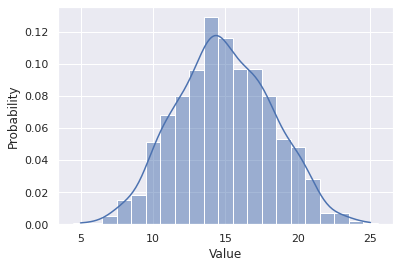
\includegraphics[width=0.85\linewidth]{"./resources/binominal.png"}
		\caption{Гистограмма биномиального распределения с $p = 0.3$, $n = 50$.}
          \label{fig:bin_dist}
	\end{center}
\end{figure}

\anonsubsection{Геометрическое распределение}

\begin{definition}
	Случайная величина $X$ имеет геометрическое распределение с
      параметром $p$ $(X\sim \Geom(p))$, если
	$$ \mathbb{P}(X = k) = (1 - p)^kp = q^k p \ , \ k \in \mathbb{N} \cup 
     \{0\}. $$
\end{definition}

Так же, как и в случае биномиального распределения, проводится некоторое
 количество испытаний Бернулли с одинаковой вероятностью успеха, до
 первого успеха. В качестве случайной величины с геометрическим распределением
 берется, как правило, количество неудач до первого успеха.

\anonsubsection{Свойство отсутствия памяти}
Случайная величина с геометрическим распределением обладает так называемым
 свойством отсутствия памяти. Неформально оно означает, что в момент проведения
 очередного испытания Бернулли количество прошлых неудач не влияет на количество
 будущих. Формально же это свойство можно сформулировать как
\newtheorem{stat}{Утверждение}
\begin{statement}
	Пусть $Y \sim \Geom(p)$, тогда $\forall m,n \in \mathbb{N} \cup 
     \{0\}$ справедливо:
	$$ 
     \mathbb{P}(Y > m + n \mid Y \ge m) = \mathbb{P}(Y > n),
     $$
\end{statement}
\begin{proof} Рассмотрим левую часть равенства:
     \begin{multline*}
          \mathbb{P}(Y > m + n \mid Y \ge m) = \dfrac{\mathbb{P}
          (Y > m + n, Y \ge m)}{\mathbb{P}(Y \ge m)} = \\
          = \dfrac{\mathbb{P}(Y > m + n)}{\mathbb{P}(Y \ge m)} = 
          \dfrac{\displaystyle\sum_{i = m + n + 1}^\infty q^i p}
          {\displaystyle\sum_{i = m}^\infty q^i p} = \dfrac{q^{m + n + 1}}{q^m} =
          q^{n + 1}.
     \end{multline*}
     С другой стороны, правая часть равна:
     $$ 
     \mathbb{P}(Y > n) = \sum_{i = n + 1}^\infty q^i p = p \dfrac{q^{n + 1}}
     {1 - q} = q^{n + 1}.
     $$
\end{proof}

Для демонстрации этого свойства в Python сгенерируем массив некоторого
 достаточного количества геометрических случаных величин. С помощью него
 построим гистограмму геометрического распределения (Рис. \eqref{subfig:geometric_distribution}). Зафиксируем некоторое $m$,
 и построим гистаграмму распределения вектора геометрических случайных
 величин из первоначального набора, значения которых больше либо равны $m$.
 В результате увидим, что при достаточно большом количестве чисел в первоначальном
 наборе гистограммы двух распределений приблизительно совпадают (Рис. \eqref{subfig:memoryless}). 

 \begin{figure}
     \centering
     \begin{subfigure}[b]{0.45\textwidth}
         \centering
         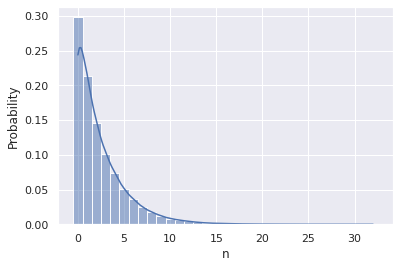
\includegraphics[width=\textwidth]{./resources/geometric.png}
         \caption{Гистограмма геометрического распределения при $p = 0.3$}
         \label{subfig:geometric_distribution}
     \end{subfigure}
     \hfill
     \begin{subfigure}[b]{0.45\textwidth}
         \centering
         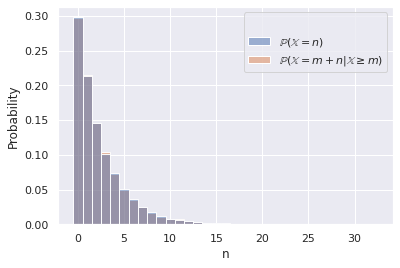
\includegraphics[width=\textwidth]{./resources/comparison.png}
         \caption{Демонстрация свойства отсутствия памяти}
         \label{subfig:memoryless}
     \end{subfigure}
     \caption{}
     \label{fig:geometric}
\end{figure}

\anonsubsection{Игра в орлянку}
Рассмотрим игру в орлянку. Для этого смоделируем последовательность
 случайных величин $X_1, X_2, \dots,$ где
$$
	X_i = 
	\begin{cases}
	     1 \ , & p = \frac{1}{2}\\
	     -1 \ , & p = \frac{1}{2}
	\end{cases}
     ,\quad i = 1,\dots,n.
$$
Тогда необходимая сумма представляется в виде:
$$
Y(i) = \dfrac{X_1 + \dots + X_i}{\sqrt n}, \quad
 i = 1,\dots,n ,
$$
где $n$ --- общее число генераций.

\begin{figure}[h]
	\begin{center}
		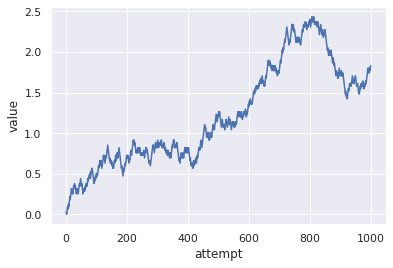
\includegraphics[width=0.75\linewidth]{"./resources/toss_game.png"}
		\caption{Траектория суммы $Y$ с $n = 1000$.}
	\end{center}
\end{figure}

Оценим $Y(n)$ при $n \to \infty$. Для этого сформулируем необходимую
 теорему.
\begin{theorem}[Центральная предельная теорема]
     Пусть $X_1,\dots, X_n,\dots$ есть бесконечная
      последовательность независимых одинаково распределенных случайных
      величин, имеющих конечное математическое ожидание $\mu$ и
      диспрерсию $\sigma^2$. Пусть также
     $$
     S_n = \displaystyle\sum_{i = 1}^n X_i
     $$
     Тогда
     $$
     \dfrac{S_n - \mu n}{\sigma \sqrt{n}} \to \Norm(0,1)
     $$
     по распределению при $n \to \infty$,
     где $\Norm(0,1)$ --- нормальное распределение с нулевым математическим ожиданием
      и стандартным отклонением, равным единице.
\end{theorem}

В случае игры Орлянки:
$$
\mu = \Exp[X_i] = 0, \quad
\sigma^2 = \Exp[(X_i - \Exp[X_i])^2] = 1, \quad i = 1, \dots, n
$$
Тогда поолучим, что последовательность случайных величин
$$
Y_n = Y(n) = \dfrac{S_n}{\sqrt{n}}
$$
Удовлетворяет условиям теоремы 1. Таким образом получаем, что $Y(n) \to \Norm(0,1)$.
\anonsection{Задание 2}
\begin{enumerate}
	\item Построить датчик сингулярного распределения, имеющий в качестве функции
     распределения канторову лесницу. С помощью критерия Колмогорова убедиться в
     корректности работы датчика.
	\item Для канторовых случайных величин проверить свойство симметричности
     относительно $\frac{1}{2}$ ($X$ и $1 - X$ распределены одинаково) и самоподобия
     относительно деления на 3 (условное распределение $Y$ при условии
     $Y \in [0, 1/3]$ совпадает с распределением $\frac{Y}{3}$) с помощью критерия
     Смирнова.
	\item Вычислить значение математическое ожидание и дисперсии для данного
     распределения. Сравнить теоритические значения с эмпирическими для разного объема
     выборок. Проиллюстрировать сходимость.
\end{enumerate}

\anonsubsection{Датчик сингулярного распределения}

\anonsection{Задание 3}
\anonsubsection{Формулировка задания}
\begin{enumerate}
	\item Построить датчик экспоненциального распределения. Проверить для
     данного распределения свойство отсутствия памяти. Пусть $X_1, X_2,
     \dots, X_n$ --- независимо экспоненциально распределенные с. в. с
     параметрами $\lambda_1, \lambda_2, \dots, \lambda_n$ соответственно.
     Найти распределение случайной величины $Y = \min(X_1, X_2, \dots, X_n)$.
	\item На основе датчика экспоненциального распределения построить датчик
     пуассоновского распределения.
	\item Построить датчик пуассоновского распределения как предел
     биномиального распределения. С помощью критерия хи-квадрат Пирсона
     убедиться, что получен датчик распределения Пуассона.
	\item Построить датчик стандартного нормального распределения методом
     моделирования случайных величин парами с переходом в полярные координаты.
     Проверить при помощи t-критерия Стьюдента равенство математических
     ожиданий, а при помощи критерия Фишера равенство дисперсий.  
\end{enumerate}

\anonsubsection{Датчик экспоненциального распределения}
\begin{definition}
	Случайная величина $X$ имеет экспоненциальное распределение с параметром
     $\lambda > 0$, если ее функция распределения имеет вид:
	\begin{equation}\label{exp_func}
	    F_X(x) = 
        \begin{cases}
	        1 - e^{-\lambda x}, &x \geqslant 0,\\
	        0, &x < 0.
	    \end{cases}
	\end{equation}
\end{definition}

\begin{theorem}[Метод обратной функции]\label{theor_inverse}
    Пусть функция распредления $ F $ имеет обратную $ F^{-1} $. Тогда
     функцией распределения случайной величины
    $$
     X = F^{-1}(Y),
    $$
     где $ Y \sim \Uni[0,1]$, является $ F $.
\end{theorem}
\begin{proof}
    Найдем функцию распределения $ X $:
    $$
     F_X(x) = \mathbb{P}(X < x) = \mathbb{P}(F^{-1}(Y) < x) =
      \mathbb{P}(Y < F(x)) = F(x).
    $$
\end{proof}

В случае экспоненциального распределения функция распределения \eqref{exp_func}
 удовлетворяет условиям теоремы и обратная к ней легко выражается:
$$
    F_X^{-1}(y) = -\frac{1}{\lambda} \ln(1 - y).
$$
Суперпозиция $ F(Y) $,где $ Y \sim \Uni[0,1] $ является случайной величиной,
 имеющей экспоненциальное распределение с параметром $ \lambda $:
$$
 X = -\frac{1}{\lambda} \ln(1 - Y) \sim \Expon(\lambda).
$$
На Рис.\eqref{fig:exp_dist} приведено сравнение полученной эмпирически,
 с помощью построенного датчика, плотности экспоненциального распределения
 и его теоретической плотности, представимой в виде:
$$
p(x) = \lambda e^{-\lambda x}
$$
при $ \lambda = 0.5 $.

 \begin{figure}[ht]
	\centering
	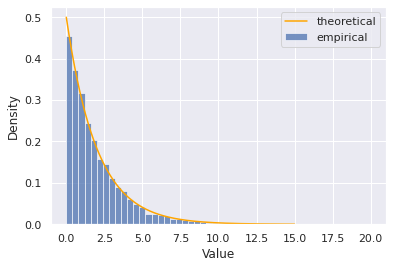
\includegraphics[width = 0.8\linewidth]{"./resources/exp_dist.png"}
	\caption{Эмпирическая и теоретическая плотности экспоненциального
     распределения при $ \lambda = 0.5 $.}
    \label{fig:exp_dist}
\end{figure}

\anonsubsection{Свойство отсутствия памяти}
Экспоненциальное распределение, как и его дискретный аналог --- геометрическое,
 обладает свойством отсутствия мапяти, которое в данном случае можно сформулировать
 как
\begin{statement}
	Случайная величина $X\sim \Expon(\lambda)$ обладает свойством отсутствия памяти,
     то есть $ \forall s,t \ge 0 $ следует, что
	\begin{equation}\label{expmem}
	    \mathbb{P} (X \ge s + t \mid X \ge t) = \mathbb{P} (X \ge s). 
	\end{equation}
\end{statement}
\begin{proof}
	$$
	\mathbb{P}(X \ge s + t \mid X \ge t) = \frac{\mathbb{P}(X \ge s + t, X \ge t}
	 {\mathbb{P}(X \ge t)} = \frac{\mathbb{P} (X \ge s + t)}{\mathbb{P}(t \ge t)}
	 = \mathbb{P}(X \ge s). 
	$$
	Таким образом, получаем:
	\begin{equation}
		\mathbb{P}(X\ge s+t)=\mathbb{P}(X\ge t)\mathbb{P}(X\ge s). \label{equi}
	\end{equation}
	Для экспоненциально распределенной случайной величины верно, что:
	$$
	\mathbb{P} (X \ge t) = 1 - F_X(t) = e^{-\lambda t}, \quad
	\mathbb{P} (X \ge s + t) = e^{-\lambda(s + t)}.
	$$
	Следовательно, для \eqref{equi} выполняется:
	$$
	e^{-\lambda(s + t)} = e^{-\lambda s} e^{-\lambda t}.
	$$
	Следовательно, экспоненциальное распределение обладает свойством отсутствия
	 памяти.
\end{proof}
На Рис.\eqref{fig:exp_memoryless}, аналогично геометрическому распределению,
 данное свойство проиллюстрировано эмпирически.
\begin{figure}[ht]
	\centering
	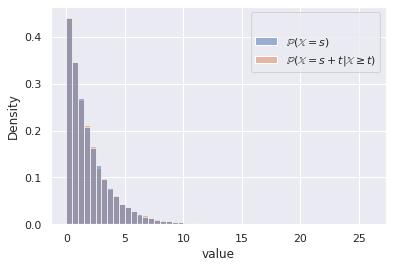
\includegraphics[width = 0.8\linewidth]{"./resources/exp_memoryless.png"}
	\caption{Эмпирическая иллюстрация свойства отсутствия памяти при t = 2.}
    \label{fig:exp_memoryless}
\end{figure}

\anonsubsection{Случайная величина $ Y = \min(X_1, X_2, \dots, X_n) $}
\begin{statement}
	Пусть $ X_1,X_2,\ldots,X_n $ --- независимые экспоненциально распределённые
	 случайные величины с параметрами $ \lambda_1,\lambda_2,\ldots,\lambda_n $
	 соответственно. Тогда случайная величина $ Y = \min(X_1, X_2, \dots, X_n)
	 \sim \Expon \left( \sum\limits_{i = 1}^n \lambda_i \right) $.
\end{statement}
\begin{proof}
	\begin{multline*}
		F_Y(x) = \mathbb{P}(Y \le x) = 1 - \mathbb{P} (Y > x) = 1 - \mathbb{P}
		 (\min(X_1, X_2, \dots, X_n) > x) = \\
		= 1 - \mathbb{P}(X_1 > x, X_2 > x, \dots, X_n > x) = \left\{ X_1, X_2,
		 \dots, X_n \text{ независимы} \right\} = \\
		= 1 - \mathbb{P} (X_1 > x) \cdot \mathbb{P} (X_2 > x) \cdot \dots
		 \mathbb{P} (X_n > x) = \\
		= 1 - \left( 1 - F_{X_1}(x) \right) \cdot \left( 1 - F_{X_2}(x) \right) 
		\cdot \dots \cdot \left( 1 - F_{X_n}(x) \right) = \\
		= 1 - e^{-\lambda_1 x} \cdot e^{-\lambda_2 x} \cdot \dots \cdot
		 e^{-\lambda_n x} = 1 - e^{-\left( \sum_{i=1}^n \lambda_i \right) x}.
	\end{multline*}
\end{proof}
Эмпирическая демонстрация этого факта для n = 4, и случайно сгенерированных
 в интервале от 0 до 0.1 параметров $\lambda_i $ приведена на Рис.\eqref{fig:exp_min}.
\begin{figure}[ht]
	\centering
	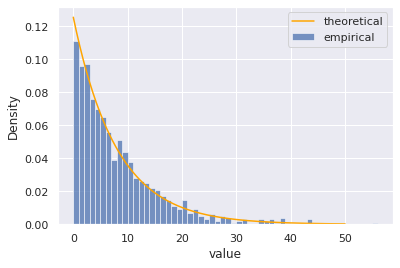
\includegraphics[width = 0.8\linewidth]{"./resources/exp_min.png"}
	\caption{Расределение $ Y = \min(X_1, \dots, X_n) $.}
    \label{fig:exp_min}
\end{figure}

\anonsubsection{Датчик пуассоновского распределения}
\begin{definition}
	Случайная величина $X$ имеет распределение Пуассона с параметром $\lambda>0$,
	 если
	$$
	\mathbb{P}(X = k) = \frac{\lambda^k}{k!} e^{-\lambda}, \quad k \in \mathbb{N} 
	\cup \{0\}.
	$$
\end{definition}
Удобный метод построения датчика пуассоновского распределения даёт следующая 
\begin{theorem}\footnote{Доказательство теоремы можно найти в \cite{model_randoms}
	 на стр. 34.}
	Пусть $X_1,X_2,\ldots,X_n,\ldots\sim Exp(\lambda)$ --- независимые одинаково
	 распредленные случайные величины. Тогда случайная величина, определенная
	 следующим образом:
	$$
	Y = \max(n \mid S_n = X_1 + X_2 + \dots + X_n < 1)
	$$
	имеет распределение Пуассона с параметром $\lambda$. При этом полагается $Y=0$,
	 если таких $ n $ не существует.
\end{theorem}
 Таким образом для моделирования случайной величины Пуассона можно последовательно
 генерировать показательные случайные величины, пока их сумма не станет больше
 единицы. Количество сгенерированных экспоненциальных величин минус один и будет
 значением пуассоновской случайной величины. На Рис.\eqref{fig:pois_dist} изображено
 сравнение распределения выборки полученной с помощью построенного вышеописанным
 способом датчика и теоретической функции вероятности.

\begin{figure}[ht]
	\centering
	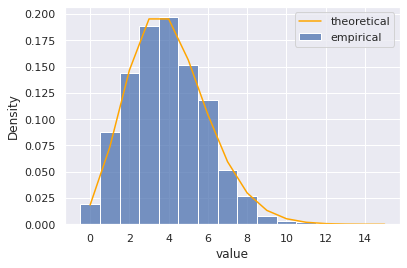
\includegraphics[width = 0.8\linewidth]{"./resources/pois_dist.png"}
	\caption{Эмпирическая и теоретическая плотности распределения Пуассона при
	 $ \lambda = 4 $.}
    \label{fig:pois_dist}
\end{figure}

\anonsubsection{Датчик пуассоновского распределения как предел биномиального 
 распределения}
Другой способ моделирования пуассоновской случайной величины основывается на 
 следующей предельной теореме, связывающей распределение Пуассона с биномиальным
 распределением.
Пусть
$$
P_n(k) = 
\begin{cases}
	C_n^k p^k q^{n-k}, & k = 0, 1, \dots, n,\\
	0, & k = n + 1, n + 2, \dots, 
\end{cases}
$$
и пусть $ p $ является функцией от $ n, \ p = p(n) $.
\begin{theorem}[Пуассона]\footnote{Доказательство этой теоремы можно найти в
	 \cite{shir_prob} на стр. 90.}
	Пусть $ p(n) \to 0, n \to \infty $, причем так, что $ n p(n) \to \lambda $,
	 где $ \lambda > 0 $. Тогда для любого $ k = 0, 1, \dots $
	$$
	P_n(k) \to \dfrac{\lambda^k e^{-k}}{k!}, \quad k = 0, 1, \dots .
	$$
\end{theorem}
Таким образом строить датчик распределения Пуассона с параметром $ \lambda $
 можно с помощью датчика биномиального распределения при $ p =
 \dfrac{\lambda}{n} $ и больших значениях $ n $. На Рис.\eqref{fig:pois_binlim}
 проиллюстрировано достаточно хорошее совпадение распределений $ \Bin\left( n,
 \dfrac{\lambda}{n} \right) $ и $ \Pois(\lambda) $ при $ n = 10000, \lambda = 10 $.

\begin{figure}[ht]
	\centering
	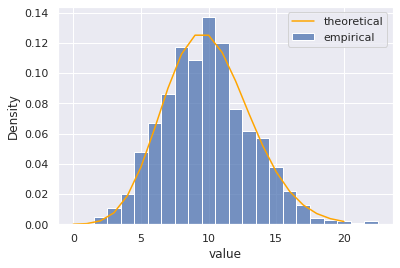
\includegraphics[width = 0.8\linewidth]{"./resources/pois_binlim.png"}
	\caption{Демонстрация предельного совпадения биномиального и пуассоновского
	 распределений при $ n = 10000, \lambda = 10 $.}
    \label{fig:pois_binlim}
\end{figure}

\anonsubsection{Проверка корректности датчика и критерий хи-квадрат Пирсона}
Проверим корректность построенного с помощью биномиального распределения датчика.
 Для этого воспользуемся криетрием хи-квадрат Пирсона, но для начала дадим
 необходимые определения.
\begin{definition}
	Пусть случайные величины $ Z_1, \dots, Z_k $ распределены по стандартному
	 нормальному закону $ \mathcal{N}(0,1) $ и независимы. Тогда распределние
	 случайной величины $ R_k^2 = Z_1^2 + \dots + Z_k^2 $ называют распределением
	 хи-квадрат с $ k $ степенями свободы(кратко: $ R_k^2 \sim \chi_k^2) $. 
\end{definition}
Пусть $ X_1, \dots, X_n $ --- выборка из закона с функцией распределения $ F(x) $.
 Разобьем множество значений $ X_1 $ на $ N $ промежутков(возможно бесконечных)
 $ \delta_j = (a_j, b_j], \quad j = 1, \dots, N$. В случае дискретных распределений
 вместо промежутков значений можно рассматривать отдельные значения. 
 Положим $ p_j = \mathbb{P}(X_1 \in \delta_j) $, а случайные величины $ \nu_j $ ---
 равными количеству элементов выборки в $ \delta_j \ (\nu_1 + \dots + \nu_N = n) $.
 Функция $ F $ неизвестна и проверяется гипотеза
$$
 H_0: F(x) = F_0(x),
$$
 где $ F_0 $ --- заданная функция распределения. Если гипотеза верна, то согласно
 закону больших чисел частоты попадания в промежутки $ \hat{p}_j = \dfrac{\nu_j}{n} $
 при достаточно больших $ n $ должны быть близки к соответствуюшим вероятностям
 $ p_j^0 = F_0(b_j) - F_0(a_j) $. В качетсве меры отклонения от гипотезы $ H_0 $
 принимается статистика
$$
X_n^2 = n \sum_{j = 1}^N \frac{1}{p_j^0}(\hat{p}_j - p_j^0)^2 = \sum_{j = 1}^N
 \frac{(\nu_j - np_j^0)^2}{np_j^0},
$$
которая по сути является взвешенной суммой квадратов отклонений частот от
 гипотетических вероятностей. В силу центральной предельной теоремы
 каждое отклонение асимптотически нормально и имеет порядок малости
 $ \dfrac{1}{\sqrt{n}} $, поэтому представляется правдоподобной следующая
\begin{theorem}\footnote{ Доказательство этой теоремы можно найти в
	 \cite{lagutin_stat} на стр. 274.}
	Если $ 0 < p_j^0 < 1, \quad j = 1, \dots, N,$ то при $ n \to \infty $
	$$
	X_n^2 \xrightarrow{d} \zeta \sim \chi_{N-1}^2.
	$$
\end{theorem}
Здесь сходимость понимается в смысле сходимости по распределению. Аналогично теореме
 Колмогорова, данная теорема позволяет оценивать вероятность отклонения, задаваемого
 статистикой Пирсона, посчитанного для конкретной выборки и, в зависимости от
 необходимого уровня значимости, принимать или отвергать гипотезу $ H_0 $.

\anonsubsection{Датчик стандартного нормального распределения методом моделирования
 случайных величин парами с переходом в полярные координаты}
\begin{definition}
	Случайная величина $ X $ имеет нормальное распределение вероятностей с параметрами
	 $ \mu $ и $ \sigma^2 $, $ X \sim \mathcal{N}(\mu,\sigma^2) $ ($ \mu $ ---
	 математическое ожидание $ X $, $ \sigma^2 $ --- дисперсия $ X $), если ее плотность
	 распределения задается формулой
	$$
	p_{X}(x) = \frac{1}{\sqrt{2\pi}\sigma} e^{-\frac{(x - a)^2} {2 \sigma^2}},
	 \quad -\infty < x < +\infty.
	$$
\end{definition}
\begin{definition}
	Нормальное распределение с параметрами $ a = 0 $ и $ \sigma^2 = 1 $ называется
	 стандартным нормальным распределением, и ее плотность распределения имеет
	 следующий вид:
	$$
	p_{X}(x) = \frac{1}{\sqrt{2\pi}} e^{-\frac{x^2}{2}}, \quad
	 -\infty < x < \infty.
	$$
\end{definition}
Рассмотрим способ точного моделирования, базирующийся на нелинейном преобразовании
 пары независимых равномерно распределенных на $ [0,1] $ случайных величин
 $ \eta_1, \eta_2 $ в пару независимых $ \mathcal{N}(0,1) $ случайных величин
 $ X, Y $:
 $$
 X = \sqrt{-2 \ln\eta_1} \cos(2 \pi \eta_2), \quad Y = \sqrt{-2 \ln \eta_1}
 \sin(2 \pi \eta_2)
 $$
\begin{proof}
	Для независимых $ \mathcal{N}(0,1) $ случайных величин $ X $ и $ Y $
	 плотность вектора $ (X,Y) $ служит
	$$
	p_{(X,Y)}(x,y) = \frac{1}{\sqrt{2 \pi}} e^{-\frac{x^2}{2}}
	 \frac{1}{\sqrt{2 \pi}} e^{-\frac{y^2}{2}} = \frac{1}{2 \pi}
	 e^{-\frac{x^2 + y^2}{2}}.
	$$
	Обозначим через $ R $ и $ \varPhi $ полярные координаты точки $ (X, Y): X =
	 R \cos \varPhi, \ Y = R \sin \varPhi $. Воспользуемся далее формулой
	 преобразования плотности:
	$$
	p_{\eta}(y) = |J(y)| p_{\xi}(f^{-1}(y)),
	$$
	где 
	$
	J(y) = \det
 	\begin{pmatrix}
  		\frac{\partial f_1^{-1}}{\partial y_1} & \dots & \frac{\partial f_k^{-1}}
		 {\partial y_1} \\
  		\dots  & \dots  & \dots \\
  		\frac{\partial f_1^{-1}}{\partial y_k} & \dots & \frac{\partial f_k^{-1}}
		 {\partial{y_k}}
	\end{pmatrix}
	$ --- якобиан $ f^{-1} $. \medskip\\ 
	Находим(в данном случае якобиан замены равен $ r $) 
	$$
	p_{(R, \varPhi)}(r, \varphi) = \frac{1}{2 \pi} e^{-\frac{r^2}{2}} r, \quad r > 0,
	 \ 0 < \varphi < 2 \pi.
	$$
	Так как она распадается в произведение плотностей 
	$$ 
	p_R(r) = r e^{-\frac{r^2}{2}} \mathbb{I}_{\{r > 0 \}} \ \text{и} \
	 p_{\varPhi}(\varphi) = \dfrac{1}{2 \pi} \mathbb{I}_{\{0 < \varphi < 2 \pi\}},
	$$ 
	то $ R $ и $ \varPhi $ независимы. Интегрируя плотности,
	 вычисляем функцию распределения 
	$$ 
	F_R(r) = 1 - e^{-\dfrac{r^2}{2}}, \quad \text{при} \ r \ge 0 \ \text{и} \
	 F_{\varPhi}(\varphi) = \dfrac{\varphi}{2 \pi}, \quad \text{при} \ 0 \le \varphi
	 \le 2 \pi.
	$$
	Методом обратной функции (Теорема 4) получаем формулы для моделирования случайных
	 величин $ R $ и $ \varPhi : \ R = \sqrt{-2 \ln \eta_1}, \ \varPhi = 2 \pi \eta_2, $
	 которые остается подставить в формулы замены координат.
\end{proof}
Будем генерировать стандартные номально-распределенные случайные величины с помощью
 полученных явно их выражений. Сравнение плотности полученной выборки и теоретической
 плотности приведено на Рис.\eqref{fig:norm_pair}.

\begin{figure}[ht]
	\centering
	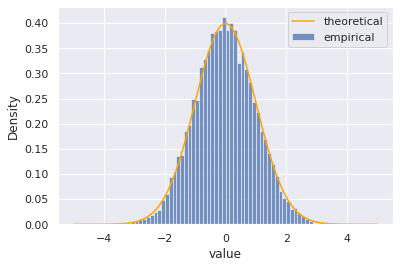
\includegraphics[width = 0.8\linewidth]{"./resources/norm_pair.png"}
	\caption{Демонстрация совпадения сгенерированного стандартного нормального
	 распределения с теоретическим при размере выборки $ n = 10000 $.}
    \label{fig:norm_pair}
\end{figure}

\anonsubsection{Критерий Фишера и t-критерий Стьюдента}
Проверим равенство дисперсий и матожиданий пары случайных величин построенных с
 помощью такого датчика. Для этого воспользуемся критерием Фишера и t-критерием
 Стьюдента.
\begin{definition}
	Случайная величина $ \zeta $ имеет $ F $-распределение(Фишера-Снедекора) с 
	 $k_1$ и $k_2$
	 степенями свободы(обозначается $ \zeta \sim F_{k_1,k_2}$), если
	$$
	 \zeta = \left. \left( \dfrac{1}{k_1} \xi \right) \right/ \left( \dfrac{1}{k_2}
	  \eta \right),
	$$
	где $ \xi \sim \chi_{k_1}^2, \ \eta \sim \chi_{k_2}^2 $, $ \xi $ и $ \eta $
	 независимы.
\end{definition}

\begin{definition}
	Пусть случайные величины $ Z $ и $ R_k^2 $ независимы и распределены согласно
	 законам $ \mathcal{N}(0,1) $ и $ \chi_k^2 $ соответственно. Тогда распределение
	 случайной величины $ T_k  = Z / \sqrt{R_k^2 / k} $ называют
	 распределением Стьюдента с k степенями свободы или t-распределением
	 (кратко $ T_k \sim t_k $).
\end{definition}

Критерий Фишера по сути может быть сформулирован следующим образом.
Если гипотеза $ H': \sigma_1 = \sigma_2, \ \mu_1 $ и $ \mu_2 $ --- любые 
 верна, то статистика $ S_1^2 / S_2^2 $ распределена по закону
 $ F_{n-1,m-1} $. Здесь
$$
S_1^2 = \frac{1}{n - 1} \sum_{i = 1}^{n}(X_i - \overline{X})^2, \quad
S_2^2 = \frac{1}{m - 1} \sum_{i = 1}^{m}(Y_i - \overline{Y})^2
$$
--- несмещенные оценки для дисперсий $ \sigma_1^2 $ и $ \sigma_2^2 $.
Это утверждение опирается на определение распределения Фишера и следующую теорему.
\begin{theorem}\footnote{Доказательство этой теоремы можно найти в
	\cite{lagutin_stat} на стр. 149.}
	Для нормальной выборки $ X_i \sim \mathcal{N}(\theta_1, \theta_2^2) $ Выборочное
	 среднее $ \overline{X} = \frac{1}{n}\sum X_i $ и выборочная дисперсия
	 $ S^2 = \frac{1}{n} \sum (X_i - \overline{X})^2 $ независимы, причем
	 $ n S^2 / \theta_2^2 \sim \chi_{n-1}^2 $, а $\sqrt{n - 1}
	 (\overline{X} - \theta_1) / S \sim t_{n-1} $.
\end{theorem}
В силу этой теоремы $ (n-1) S_1^2 / \sigma_1^2 \sim \chi_{n-1}^2,
 \ (m - 1) S_2^2 / \sigma_2^2 \sim \chi_{m-1}^2 $, и следовательно
 формулировка критерия Фишера верна. Отметим, что критерий Фишера имеет
 двустороннюю критическую область, поэтому сравнение статистики для отвержения
 или принятия гипотезы в этом случае нужно проводить и с $ \dfrac{\alpha}{2} $
 - квантилью и с $ 1 - \dfrac{\alpha}{2} $ - квантилью распределения
 Фишера-Снедекора. \medskip\\
Проверим теперь равенство математических ожиданий с помощью критерия Стьюдента.
 Обозначим неизвестную общую дисперсию через $ \sigma^2 $. Так как распределение
 хи-квадрат является частным случаем гамма-распределения $(\chi_k^2 
 \sim \Gamma(k/2, 1/2)) $, получаем
$$
 \sigma^{-2} \left[(n - 1) S_1^2 + (m - 1) S_2^2 \right] \sim \chi_{n + m - 2}^2.
$$
Поскольку математическое ожидание закона $ \chi_{n + m - 2}^2 $ равно $ n + m - 2 $,
 статистика $ S_{tot}^2 = \left[(n - 1) S_1^2 + (m - 1) S_2^2 \right] / (n + m -2) $
 несмещенно оценивает $ \sigma^2 $ по объединенной выборке.

При справедливости гипотезы $ H^{''}: \mu_1 = \mu_2 $ ввиду независимости выборок
 имеем: $\overline{X} - \overline{Y} \sim \mathcal{N}(0, (1/n + 1/m)\sigma^2) $.
 Отсюда согласно определению закона Стьюдента:
$$
T = \left( \overline{X} - \overline{Y} \right) \left/ \left( S_{tot}
 \sqrt{\dfrac{1}{n} + \dfrac{1}{m}} \right) \right. = \left. \sqrt{\dfrac{nm}{n + m}} \left(\overline{X}
 - \overline{Y} \right) \right/ S_{tot} \sim t_{n + m - 2}.
$$
Это приводит к критерию Стьдента, позволяющему проверить гипотезу $ H^{''} $.
 Отметим также, что данный критерий, как и критерий Фишера имеет двустороннюю критическую
 область.
\anonsection{Задание 4}
\anonsubsection{Формулировка задания}
\begin{enumerate}
\item Построить датчик распределения Коши. 
\item На основе датчика распределения Коши с помощью метода фон Неймана построить
 датчик стандартного нормального распределения. При помощи функции normal
 probabitity plot убедиться в корректности построенного датчика и обосновать
 наблюдаемую линейную зависимость.
\item Сравнить скорость моделирования стандартного нормального распределения в
 заданях 3 и 4.
\end{enumerate}

\anonsubsection{Датчик распределения Коши}
\begin{definition}
	Случайная величина $X$ имеет распределение Коши с параметрами $a$ и $b$, если
     ее функция распределения имеет вид:
    $$
	F_X(x) = \frac{1}{\pi}\arctan\left(\frac{x - a}{b}\right) + \frac{1}{2}.
	$$
	Плотность распределения Коши:
	$$
	p_X(x) = \frac{1}{\pi}\frac{b}{(x- a)^2 + b^2}.
	$$
\end{definition}

Функция распределения $F_X(x)$ обладает обратной, а значит в данном случае для
 моделирования распределения можно пользоваться методом обратной функции
 (Теорема \eqref{theor_inverse}). Обратная функция для $F_X(x)$ равна $F_X^{-1}(y)
 = a + b\tan\left(\pi\left(y - \frac{1}{2}\right)\right)$. Следовательно,
 в качестве датчика распределения Коши можно построить датчик случайной величины
 $X = F_X^{-1}(Y)$, где $Y \sim U[0, 1]$. На Рис.\eqref{fig:cauchy_ecdf}
 продемонстрировано совпадение эмпирической и теоретической функций распределения
 для распределения Коши, полученного построенным датчиком.

\begin{figure}[ht]
	\centering
	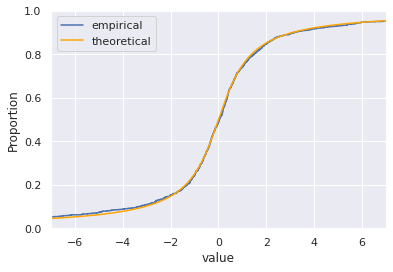
\includegraphics[width = 0.7\linewidth]{"./resources/cauchy_ecdf.png"}
	\caption{Демонстрация совпадения эмпирической и теоретической функций
     распределения для распределения Коши. Размер выборки: $ n = 1000 $.}
    \label{fig:cauchy_ecdf}
\end{figure}

\anonsubsection{Метод фон Неймана}
Метод фон Неймана заключается в моделировании нормального распределения путём
 мажорирования плотностью распределения Коши с параметрами $a$ и $b$. Для достижения
 наилучшей оценки, будем подбирать параметры $a$ и $b$. \\
Плотность стандартного нормального распределения $p_1(x)$ и плотность распределения
 Коши $p_2(x)$ выглядят следующим образом:
$$
    p_1(x) = \frac{1}{\sqrt{2\pi}}e^{-\frac{x^2}{2}},
$$

$$
    p_2(x) = \frac{1}{\pi}\frac{b}{(x - a)^2 + b^2}.
$$

При моделировании будем следовать алгоритму:
\begin{enumerate}
	\item возьмем некоторое число $k > 0$, такое что $p_1(x) \leq kp_2(x),
     \forall x\in \mathbb{R}$,
	\item рассмотрим значение случайной величины $x = X, X\sim Cauchy(a, b)$,
	\item сгенерируем случайную величину $y = Y(x)\sim Bern\left(\frac{p_1(x)}
     {kp_2(x)}\right)$,
	\item если $y = 1$, то $x$ --- значение из распределения с плотностью $p_1(x)$,
     иначе --- продолжаем моделирование, начиная с пункта 2).
\end{enumerate}
Данный алгоритм работает тем быстрее, чем ближе отношение $\frac{p_1(x)}{kp_2(x)}$
 к единице, поэтому в качестве $k$ возьмем $k^* = \min\limits_{a, b}
 \max\limits_x\frac{p_1(x)}{p_2(x)}$.
Рассмотрим отношение 
$$
    \frac{p_1(x)}{p_2(x)} = \frac{\sqrt{\pi}}{\sqrt{2}b}e^{-\frac{x^2}{2}} 
     \left((x - a)^2 + b^2\right).
$$
Пусть $a = 0$. Рассмотрим вспомогательную функцию:
$$
    g(x) = e^{-\frac{x^2}{2}} \left( x^2 + b^2 \right).
$$
Найдем максимум этой функции:
$$
    g'(x) = e^{-\frac{x^2}{2}} x \left( 2 - b^2 - x^2 \right) = 0,
$$
следовательно, точки экстремума:
$$
    \left[
    \begin{aligned}
        x = 0, |b| > \sqrt{2},\\
        x = \pm\sqrt{2 - b^2}, 0 < |b| \leq \sqrt{2}.
    \end{aligned}
    \right.
$$
Таким образом,
$$
    k* = \min \left\{ \min_{|b| > \sqrt{2}} \sqrt{\frac{\pi}{2}} b,\;
     \min_{0 < |b| < \sqrt{2}} \frac{\sqrt{2\pi}}{b}e^{\frac{b^2}{2} - 1} \right\}.
$$
Поскольку $k > 0$, то и $b > 0$. Найдем максимум вспомогательной функции
$$
    h(b) = \frac{e^{\frac{b^2}{2} - 1}}{b}:
$$

$$
    h'(b) = \frac{1-b^2}{b^2}e^{\frac{b^2}{2} - 1},
$$

следовательно, поскольку $b > 0$, точкой экстремума является $b = 1$.\\
Получаем оптимум при $a^* = 0,\, b^* = 1:$
$$
    k^* = \min\left\{\sqrt{\pi}, \sqrt{\frac{2\pi}{e}}\right\} = 
     \sqrt{\frac{2\pi}{e}}.
$$
Докажем, что $a = 0$ --- оптимальное значение параметра.
\begin{multline}
    k^* = \min_{a, b} \max_x \left( \frac{\sqrt{\pi}}{\sqrt{2}b} e^{-\frac{x^2}{2}}
     \left((x - a)^2 + b^2\right)\right) = \\
    = \min_a\left\{\min_{b > \sqrt{2}}\left.\frac{p_1(x)}{p_2(x)}\right|_{x = 0},
     \left.\min_{0 < b\leq\sqrt{2}}\frac{p_1(x)}{p_2(x)}\right|_{x =
     \pm\sqrt{2 - b^2}}\right\} > \\
    > \min_a\left\{min_{b > \sqrt{2}}\frac{\sqrt{\pi}}{\sqrt{2}b}
     \left(a^2 + b^2\right), \min_{0 < b \leq \sqrt{2}} \left( \sqrt{2 - b^2} +
     |a|\right)\right\}
\end{multline}
Минимум выражения достигается при $a = 0$.

Иллюстрация работы построенного датчика, использующая Python функцию
 scipy.stats.probplot, представлена на Рис. \eqref{fig:norm_probplot}. На оси ординат
 откладываются точки выборки, на оси абсцисс --- квантили стандартного нормального
 распределения. Прямой линии соответствует "точное"  нормальное распределение,
 наилучшим образом приближающее, в смысле указанных осей, значения выборки. Видно, 
 что полученная с помощью датчика Фон-Неймана выборка следует стандартному нормальному
 распределению.

\begin{figure}[ht]
	\centering
	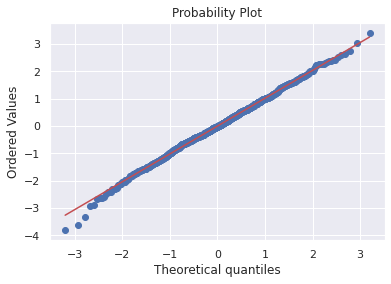
\includegraphics[width = 0.7\linewidth]{"./resources/norm_probplot.png"}
	\caption{Демонстрация совпадения построенного с помощью метода Фон-Неймана
     распределения со стандартным номральным при размере выборки $ n = 1000 $.}
    \label{fig:norm_probplot}
\end{figure}

 Возьмем далее случайную величину  \( \xi\sim N(\mu,\sigma^2) \). Ее функция
 распределения
$$
	F_{\xi}(x) = \dfrac{1}{\sqrt{2\pi\sigma^2}} \int\limits_{-\infty}^x
     e^{-\dfrac{(t - \mu)^2}{2 \sigma^2}} dt
$$
Введем замену переменной $ s = \dfrac{t - \mu}{\sigma} $. Тогда
$$
	F_{\xi}(x) = \dfrac{1}{\sqrt{2\pi}} \int\limits_{-\infty}^{\frac{x - \mu}
     {\sigma}} e^{-\dfrac{s^2}{2}} ds = F \left( \dfrac{x - \mu}{\sigma} \right) 
$$
где \( F(x) \) --- функция стандартного нормального распределения.

Таким образом, квантили различных распределений связаны между собой линейно, что
 означает, что любую нормальную случайную величину \( \xi \sim N(\mu, \sigma^2) \)
 можно представить в виде \( \xi = \sigma \eta + \mu \), где \( \eta \sim N(0,1) \),
 а прямая в функции probplot будет прямой со сдвигом \( \mu \) и с коэффициентом
 наклона \( \sigma \).

\anonsubsection{Сравнение времени работы}
На Рис. \eqref{fig:times} приведен график сравнения скорости работы датчика
 стандартного нормального распределения с моделированием случайных величин парами
 и датчика, построенного методом Фон-Неймана.

\begin{figure}[ht]
	\centering
	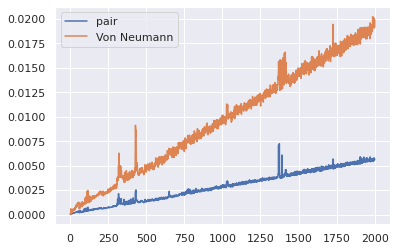
\includegraphics[width = 0.7\linewidth]{"./resources/times.png"}
	\caption{Зависимость времени моделирования от размера генерируемой выборки.}
    \label{fig:times}
\end{figure}
\anonsection{Задание 5}
\anonsubsection{Формулировка задания}
\begin{enumerate}
	\item Пусть $X_i \sim N(\mu, \sigma^2)$. Убедиться эмпирически в справедливости
     ЗБЧ и ЦПТ, т.е. исследовать поведение суммы $S_n$ и эмпирического распределения
     величины
	\begin{equation*}
	\sqrt{n} \left( \frac{S_n}{n} - a \right).
	\end{equation*}
	\item Считая $ \mu $ и $ \sigma^2 $ неизвестными, для пункта 1 построить
     доверительные интервалы для среднего и дисперсии.
	\item Пусть $ X_i \sim K(a, b) $ имеет распределение Коши со сдвигом $ a $ и
     масштабом $ b $. Проверить эмпирически, как ведут себя суммы $S_n/n$.
     Результат объяснить, а также найти закон распределения данных сумм.
\end{enumerate}

\anonsubsection{Закон больших чисел и центральная предельная теорема для нормального
 распределения}
Пусть $X_i\sim\mathcal{N}(\mu,\sigma^2)$. Исследуем поведение суммы $\dfrac{S_n}{n}$
 и эмпирического распределения величины
$$
 \sqrt{n}\left(\dfrac{S_n}{n}-\mu\right).
$$
\begin{theorem}[Закон больших чисел]
	Пусть $X_1,X_2,\ldots$ --- независимые одинаково распределенные случайные величины,
	 $\mathbb{E} X_i = \mu ,\ \forall i \in \mathbb{N},\ | \mu | < \infty ,\ S_n = X_1 +
	 \dots + X_n $.
	Тогда
	 $ \dfrac{S_n}{n} \xrightarrow[n \to \infty]{\mathbb{P}} {}\mu $, т.~е.
	$$
	 \forall \varepsilon > 0 \quad \mathbb{P} \left( \left| \dfrac{S_n}{n} - \mu \right|
	 \ge \varepsilon \right) \xrightarrow [n \to \infty] {}0.
	$$
\end{theorem}
\begin{theorem}[Центральная предельная теорема]
	Пусть $ X_1, X_2, \dots $ --- независимые одинаково распределенные случайные
	 величины, $ 0 < \Exp X_i^2 < \infty,\ \forall i \in \mathbb{N},\ S_n = X_1 
	 + \dots + X_n $.
	Тогда
	$$
	 \mathbb{P} \left( \dfrac{S_n - \mathbb{E} S_n}{\sqrt{\mathbb{D} S_n}} \leq x \right) 
	 \xrightarrow [n \to \infty]{} \Phi(x), \quad x \in \mathbb(R),
	$$
	где $\Phi(x)$ --- функция стандартного нормального распределения:
	$$
	 \Phi(x) = \dfrac{1}{\sqrt{2\pi}} \int\limits_{-\infty}^x e^{-\frac{t^2}{2}} dt.
	$$
\end{theorem}
Доказательство этих теорем представлено в \cite{shir_prob}. На рисунке
 \eqref{fig:law_of_large_numbers} представлена иллюстрация сходимости из закона
 больших чисел. На рисунке \eqref{fig:central_limit_theorem} в свою очередь
 проиллюстрирована сходимость из центральной предельной теоремы. 
\begin{figure}[ht]
	\centering
	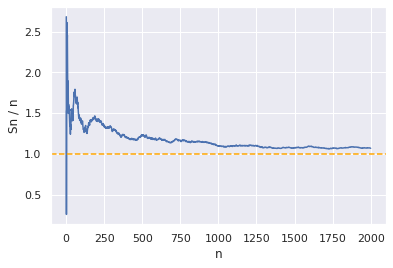
\includegraphics[width = 0.7\linewidth]{"./resources/law_of_large_numbers.png"}
	\caption{Иллюстрация сходимости среднего $ S_n / n $ к матожиданию $ \mu = 1 $ при
	 увеличени $ n $.}
    \label{fig:law_of_large_numbers}
\end{figure}

\begin{figure}[ht]
	\centering
	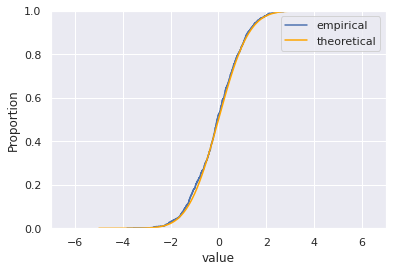
\includegraphics[width = 0.7\linewidth]{"./resources/central_limit_theorem.png"}
	\caption{Эмпирическая функция распределения величины $ \frac{S_n - \mu * n}{\sigma
	 \sqrt{n}} $ при $ n = 1000 $ и теоретическая функция распределения стандартного
	 нормального распределения.}
    \label{fig:central_limit_theorem}
\end{figure}

\anonsubsection{Доверительные интервалы для матожидания и дисперсии}
Построим доверительные интервалы для матожидания и дисперсии, считая их неизвестными.
 Случайная величина
$$
 T = \dfrac{\overline{X} - \mu}{S / \sqrt{n}},
$$
где 
$$
 S^2 = \dfrac{1}{n - 1} \displaystyle\sum_{i = 1}^n(X_i - \overline{X})
$$
--- уже встречавшаяся ранее, несмещенная оценка дисперсии, имеет распределение
 Стьюдента с $ n - 1 $ степенями свободы. Тогда, в силу симметрии распределения,
 получим:
$$
 \mathbb{P} \left( -t_{1 - \frac{\alpha}{2}} \leq T \leq t_{1 -
 \frac{\alpha}{2}} \right) = 1 - \alpha
$$
или же
$$
 \mathbb{P} \left( \overline{X} - t_{1 - \frac{\alpha}{2}} \frac{S}{\sqrt{n}}
 \leq \mu \leq \overline{X} + t_{1 - \frac{\alpha}{2}} \frac{S}{\sqrt{n}} \right)
 = 1 - \alpha,
$$
что непосредственно дает доверительный интервал для матожидания с уровнем доверия
 $ 1 - \alpha $.

Для построения доверительного интервала для дисперсии рассмотрим случайную величину
$$
 H = \dfrac{(n-1)S^2}{\sigma^2},
$$
имеющую распределение хи-квадрат $ \chi_{n-1}^2 $ с $ n - 1 $ степенями свободы.
В данном случае распределение уже не обладает свойством симметрии, поэтому будем
 брать $ \frac{\alpha}{2} $ и $ 1 - \frac{\alpha}{2} $ квантили. В таком случае
 получаем:
$$
\mathbb{P} \left( \chi_{\frac{\alpha}{2}}^2 \leq H \leq \chi_{1 -
 \frac{\alpha}{2}}^2 \right) = 1 - \alpha
$$
или
$$
\mathbb{P} \left( \dfrac{(n - 1) S^2}{\chi_{\frac{\alpha}{2}}^2} < \sigma^2 <
 \dfrac{(n - 1) S^2}{\chi_{1 - \frac{\alpha}{2}}^2} \right) = 1 - \alpha,
$$
откуда немедленно получаем доверительный интервал для дисперсии с уровнем
 доверия $ 1 - \alpha $.
 
Графики доверитльных интервалов для матожидания и дисперсии в зависимости
 от размера выборки, по которой они строятся изображены на Рис.
 \eqref{fig:mean_conf_int} и Рис.\eqref{fig:var_conf_int} соответственно.

\begin{figure}[ht]
	\centering
	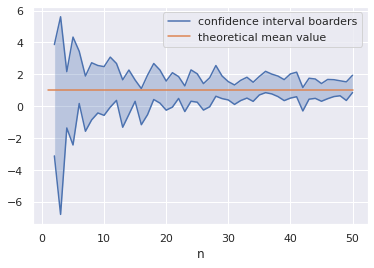
\includegraphics[width = 0.7\linewidth]{"./resources/mean_conf_int.png"}
	\caption{Эволюция доверительного интервала для матожидания $ \mu = 1 $ при
	 увеличении $ n $ с уровнем доверия 95\%.}
    \label{fig:mean_conf_int}
\end{figure}
\begin{figure}[ht]
	\centering
	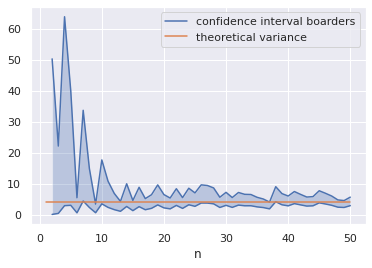
\includegraphics[width = 0.7\linewidth]{"./resources/var_conf_int.png"}
	\caption{Эволюция доверительного интервала для дисперсии $ \sigma^2 = 4 $ при
	 увеличении $ n $ с уровнем доверия 90\%.}
    \label{fig:var_conf_int}
\end{figure}

\anonsubsection{Закон больших чисел и распределение Коши}
Исследуем вопрос справедливости закона больших чисел для последовательностей случайных
 величин Коши. Эмпирически можно сделать вывод, что в отличие от выборок из нормального 
 распределения, сходимость к математическому ожиданию в данном случае отсутствует.
 Это можно объяснить тем, что у распределения Коши вовсе нет математического ожидания,
 а выборочное среднее в выборке из таких случайных величин также будет распределена
 по закону Коши. Иными словами, если $ X_1, \dots, X_n \sim C(a,b) $, то
$$
 \overline{X} = \dfrac{\sum_{i = 1}^n X_i}{n} \sim C(a, b).
$$
Это свойство доказывается с помощью характеристических функций.
\begin{definition}
	Функция $ \phi_X(t) = \Exp e^{itX} $ вещественного переменного $ t $ называется
	 характеристической функцией случайной величины $ X $.
\end{definition}
\begin{statement}
	Характеристическая функция суммы независимых случайных величин равна произведению
	 функций слагаемых.
\end{statement}
\begin{proof}
	Если случайные величины $ X $ и $ Y $ независимы, то, по свойству математческих 
	ожиданий получаем:
	$$
	 \phi_{X + Y}(t) = \Exp e^{it(X+Y)} = \Exp e^{itX} e^{itY} = \phi_X(t) \phi_Y(t).
	$$
\end{proof}
Характеристическая функция однозначно задает распределение, то есть если две случайные
 величины имеют одинаковые характеристические функции, то их распределения совпадают.
 В таком случае, рассмотрим характеристическую функцию выборочного среднего и учтем при
 этом, что для $X_i \sim C(a, b),\ \phi_{X_i} = e^{ait - b|t|} $.
$$
 \psi_{\overline{X}}(t) = \phi_{X_1 + \dots + X_n}\left( \frac{t}{n} \right) = 
  \left( \phi_{X_1(\frac{t}{n})} \right)^n = \left( e^{\frac{ait - b|t|}{n}} \right)^n = 
  \phi_{X_1}(t).
$$
То есть получаем, что $ \overline{X} \sim C(a, b) $. Отсутствие сходимости выборочного
 среднего проиллюстрировано на рисунке \eqref{fig:cauchy_law_of_large_numbers}. На рисунке
 \eqref{fig:sample_mean_cauchy_cdf} проилюстрировано совпадение распределений Коши и
 выборочного среднего для выборки из распределения Коши(так называемого свойства
 устойчивости).
\begin{figure}[ht]
	\centering
	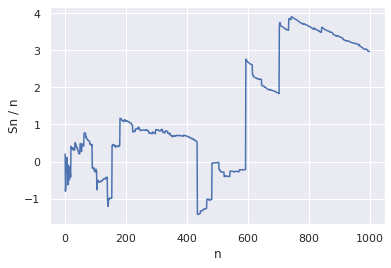
\includegraphics[width = 0.7\linewidth]{"./resources/cauchy_law_of_large_numbers.png"}
	\caption{Поведение среднего значения в выборке из распределений Коши с ростом размера
	 выборки.}
    \label{fig:cauchy_law_of_large_numbers}
\end{figure}

\begin{figure}[ht]
	\centering
	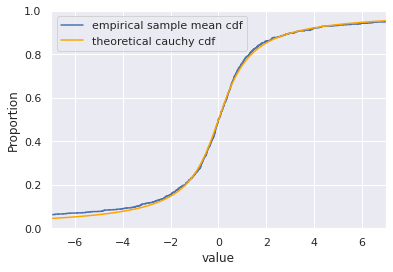
\includegraphics[width = 0.7\linewidth]{"./resources/sample_mean_cauchy_cdf.png"}
	\caption{Иллюстрация устойчивости распределения Коши: $ \overline{X} \sim C(a, b) $. 
	 $ a = 0,\ b = 1 $}
    \label{fig:sample_mean_cauchy_cdf}
\end{figure}
\anonsection{Задание 6}
\anonsubsection{Формулировка задания}
\begin{enumerate}
	\item Посчитать интеграл
	\begin{equation*}\label{integral}
	\int\limits_{-\infty}^{\infty} \int\limits_{-\infty}^\infty \cdots
     \int\limits_{-\infty}^\infty \frac{e^{-\left(x_1^2 + \ldots + x_{10}^2
     + \frac{1}{ 2^7\cdot x_1^2 \cdot \ldots \cdot x_{10}^2}\right)}}{x_1^2
     \cdot \ldots \cdot x_{10}^2}dx_1\ldots dx_{10}
	\end{equation*}
	\begin{itemize}
		\item[---] методом Монте-Карло
		\item[---] методом квадратур, сводя задачу к вычислению собственного
         интеграла Римана
	\end{itemize}
	\item Для каждого случая оценить точность вычислений.
\end{enumerate}

\anonsubsection{Метод Монте-Карло}
Перепишем интеграл
$$
\int\limits_{-\infty}^{\infty} \int\limits_{-\infty}^\infty \cdots
 \int\limits_{-\infty}^\infty \frac{e^{-\left(x_1^2 + \ldots + x_{10}^2 +
 \frac{1}{ 2^7\cdot x_1^2 \cdot \ldots \cdot x_{10}^2}\right)}}{x_1^2 \cdot
 \ldots \cdot x_{10}^2}dx_1\ldots dx_{10}
$$
в виде
$$
\int\limits_{-\infty}^{\infty} \int\limits_{-\infty}^{\infty} \ldots
 \int\limits_{-\infty}^{\infty} f(x_1,\ldots,x_{10})g(x_1,\ldots,x_{10}) dx_1
 \ldots\cdot dx_{10},
$$
где
$$
f(x) = \sqrt{\pi^{10}}\cdot \dfrac{e^{-\frac{1}{2^7\cdot x_1^2 \cdot \ldots
 \cdot x_{10}^2}}}{x_1^2\cdot \ldots \cdot x_{10}^2},\quad g(x) = \dfrac{1}
 {\sqrt{\pi^{10}}}\cdot e^{-(x_1^2+\ldots +x_{10}^2)}.
$$
Заметим, что $ g(x) $ является совместной плотностью распределения набора
 независимых случайных величин, имеющих нормальное распределение с параметрами
 $0$ и $\dfrac{1}{2}$:
$$
x=(x_1,\ldots,x_{10}),\quad x_i\sim\mathcal{N}\left(0,\dfrac{1}{2}\right).
$$
Тогда интеграл \eqref{integral} можно записать в виде:
$$
I = \mathbb{E} f(x_1,\ldots,x_{10}),\quad x_i\sim\mathcal{N}\left(0, 
 \dfrac{1}{2}\right).
$$
Рассмотрим выборку
$$
x^i = (x_1^i, \ldots, x_{10}^i),\quad x_k^i\sim\mathcal{N}\left(0,\dfrac{1}{2}
 \right),\quad k = \overline{1,10}, \quad i = \overline{1,n}.
$$
Согласно ЗБЧ выборочное среднее будет стремиться к математическому ожиданию,
 то есть:
$$
\bar{f} = \dfrac{S_n}{n} = \dfrac{1}{n} \sum_{i = 1}^n f(x^i) \xrightarrow
 [n\to\infty]{}I.
$$
Оценим погрешность метода Монте--Карло с помощью центральной предельной теоремы:
\begin{multline}\label{mc_err_estimation}
\mathbb{P} \left( \left| \dfrac{S_n}{n} - I \right| < \varepsilon \right) =
 \mathbb{P} \left( \left| \dfrac{S_n - nI}{n} \right| <\varepsilon \right) =
 \mathbb{P}\left(\left|\dfrac{S_n-nI}{\sigma\sqrt{n}}\right|<\dfrac{\sqrt{n}}
 {\sigma}\varepsilon\right) =\\
 = \mathbb{P}\left(-\dfrac{\sqrt{n}}{\sigma}\varepsilon<\dfrac{S_n-nI}
 {\sigma\sqrt{n}}<\dfrac{\sqrt{n}}{\sigma}\varepsilon\right) = \Phi_0 
 \left( \dfrac{\sqrt{n}}{\sigma}\varepsilon\right)-\Phi_0 \left( -\dfrac{\sqrt{n}}
 {\sigma} \varepsilon \right) =\\
 = \Phi_0 \left( \dfrac{\sqrt{n}}{\sigma} \varepsilon \right) - \left( 1 -
 \Phi_0 \left( \dfrac{\sqrt{n}}{\sigma} \varepsilon \right) \right) =
 2\Phi_0 \left( \dfrac{\sqrt{n}}{\sigma} \varepsilon \right)  - 1 = 2 \Phi_0(x_p) -
 1 = 1 - \alpha,
\end{multline}
где
\begin{itemize}
	\item $\Phi_0(x)$ --- функция Лапласа или функция ошибок:
	$$
	\Phi(x) = \dfrac{1}{\sqrt{2\pi}} \int\limits_{-\infty}^x e^{-\frac{t^2}{2}}dt,
	$$
	\item $x_p = \dfrac{\sqrt{n}}{\sigma} \varepsilon $ --- квантиль уровня
     $ p $. Из \eqref{mc_err_estimation} видно, что в данном случае 
     $ p = 1 - \frac{\alpha}{2} $
	\item $ \alpha $ --- уровень значимости.
\end{itemize}
Погрешность $ \varepsilon $ для соответствующего уровня значимости $ \alpha = 2 - 
 2\Phi_0(x_p)$ связана с $ x_p $ соотношением:
$$
\varepsilon = \dfrac{\sigma x_p}{\sqrt{n}}.
$$
Значение $ \sigma > 0 $ используем как значение выборочной дисперсии:
$$
\sigma = \frac{1}{n} \sum_{i = 1}^n f^2(x_i) - \left( \frac{1}{n}
 \sum_{i = 1}^n f(x_i) \right)^2.
$$
В качестве уровня значимости возьмем $ \alpha = 0.05 $:
$$
\mathbb{P} \left( \left| \dfrac{S_n}{n} - I \right| < \varepsilon \right) =
 1 - \alpha = 0.95.
$$
Ниже приведена таблица зависимости вычисленных значений интеграла и полученной
 погрешности при разном количестве испытаний:
\begin{center}
	\begin{tabular}{|c|c|c|c|}
		\hline
		Число испытаний & Результат & Погрешность&Время работы\\\hline
		$10^2$&133.0744&218.6706&0.0072\\\hline
		$10^3$&106.0557&69.5468&0.0627\\\hline
		$10^4$&111.0711&20.7890&0.5177\\\hline
		$10^5$&122.3331&6.9602&4.2440\\\hline
		$10^6$&124.8926&2.2344&42.1556 \\\hline
		$10^7$&125.0400&0.7062& 420.8312\\\hline
	\end{tabular}
\end{center}

\anonsubsection{Метод квадратур}
Сведем задачу к вычислению собственного интеграла Римана. Для этого сделаем
 следующую замену переменных:
$$
x_i = \tg \left( \frac{\pi}{2} t_i \right), t_i \in [0; 1].
$$
Таким образом, по методу прямоугольников исходный интеграл приблизится значением:
$$
I = \pi^{10} \int\limits_{0}^{1} \ldots
 \int\limits_{0}^{1} \dfrac{\exp \left\lbrace - \left( \sum\limits_{k = 1}^{10}
 \tg \left( \dfrac{\pi}{2} t_k \right)^2 + \dfrac{1}{2^7 \cdot
 \prod\limits_{k = 1}^{10} \tg \left( \dfrac{\pi}{2} t_k \right)^2} \right)
 \right\rbrace}{\prod\limits_{k = 1}^{10} \tg \left( \dfrac{\pi}{2} t_k \right)^2
 \cdot\prod\limits_{k = 1}^{10} \cos \left( \dfrac{\pi}{2} t_k \right)^2} dt_1 
 \ldots dt_{10}.
$$

Проведём равномерное разбиение отрезка \( [0,1] \) на \( N \) частей:
\[
0 = t_0 < t_1 < \ldots < t_N = 1,\quad t_i = \dfrac{i}{N}
\]

Обозначим через \( f(t_1, \ldots, t_{10}) \) подынтегральную функцию интеграла
 \( I \). Будем использовать метод средних прямоугольников. Для этого нам
 необходимо выбрать середины нашего разбиения:
\[
y_i = \dfrac{t_i + t_{i - 1}}{2},\quad i = \overline{1,N}.
\]

Тогда наш интеграл приближённо можно посчитать следующим образом:
\[
I_N = \left( \dfrac{\pi}{N} \right)^{10} \sum\limits_{i_1 = 1}^N \ldots
 \sum\limits_{i_{10} = 1}^N f(y_{i_1}, \ldots, y_{i_{10}}).
\]


Оценка погрешности метода прямоугольников на равномерной сетке имеет следующий
 вид: 
$$
\varepsilon = \dfrac{h^2}{24} (b - a) \sum\limits_{i,j = 1}^{10} \max \left|
 f''_{x_i, x_j} \right| = \dfrac{1}{6N^2} \sum\limits_{i,j = 1}^{10} \max 
 \left|f''_{x_i,x_j} \right|.
$$
Приведем таблицу зависимости результата от количества точек разбиения отрезка:
\begin{center}
	\begin{tabular}{|c|c|c|c|}
		\hline
		N & Результат & Время работы\\\hline
		3&272.6029&0.363554\\\hline
		4&183.4886&49.3912\\\hline
		5&116.3903&455.3352\\\hline
	\end{tabular}
\end{center}
\anonsection{Задание 7}
\anonsubsection{Формулировка задания}

\begin{enumerate}
	\item Методом случайного поиска найти минимальное значение функции
     $f$ на множестве $A = \{x_1, x_2 : x_1^2 + x_2^2 \leq 1\}$, т.е.
     $y = \min f(x)$, где 
\begin{equation}
    f(x) = x_1^3 \sin \left( \frac{1}{x_1} \right) + 10 x_1 x_2^4 \cos 
     \left( \frac{1}{x_2} \right)
\end{equation}
     при $ x_1 \neq 0 $ и $ x_2 \neq 0 $, функция доопределяется по
     непрерывности при $ x_1 = 0 $ или $ x_2 = 0 $.
    \item Методом имитации отжига найти минимальное значение функции
     Розенброка $ g $ в пространстве $ \mathbb{R}^2 $, где 
\begin{center}
	$ g(x) = (x_1 - 1)^2 + 100 (x_2 - x_1^2)^2 $
\end{center}
    \item Оценить точность. Сравнить результаты со стандартными методами
     оптимизации.
\end{enumerate}

\anonsubsection{Метод случайного поиска}
Возьмем единичный круг и сгенерируем на нём набор равномерно распределенных
 по нему точек. Найдем миниммальное значение.\\
Совместная плотность равномерного распределения случайных величин $ x_1,
 x_2 $ на единичном круге равна:
\begin{equation}
    f_{x_1, x_2} = \begin{cases}
        \frac{1}{\pi}, & x_1^2 + x_2^2 \leq 1,\\
        0, &\text{иначе.}
    \end{cases}
\end{equation}
В полярных координатах:
\begin{equation}
    \left\{
    \begin{array}{lll}
        x_1 = r\cos\varphi, &0 \leqslant r \leqslant 1,\\
        x_2 = r\sin\varphi, &0 \leqslant\varphi\leqslant 2\pi.\\
    \end{array}
    \right.
\end{equation}
Таким образом, получим:
\begin{equation} \label{p81}
    \mathbb{P}((x_1, x_2) \in A) = \iint \limits_{x_1^2 + x_2^2 \leq 1} 
     \frac{1}{\pi} dx_1 dx_2 = \frac{1}{\pi} \int\limits_0^1 r dr 
     \int\limits_0^{2\pi} d\varphi = \int\limits_0^1 dr^2 \int\limits_0^{2\pi}
     \frac{1}{2\pi} d\varphi.
\end{equation}
Сделаем замену
\begin{equation*}
q = r^2,\;r = \sqrt{q},\;q\in[0, 1].
\end{equation*}
Тогда выражение в \eqref{p81} примет вид:
\begin{equation}
\mathbb{P}((x_1, x_2)\in A) = \int\limits_0^1 dq\int\limits_0^{2\pi}
 \frac{1}{2\pi}d\varphi.
\end{equation}
Следовательно, $x_1$ и $x_2$ выражаются в виде:
\begin{equation*}
\left\{
\begin{array}{lll}
x_1 = \sqrt{q}\cos\varphi, &q\sim U[0, 1],\\
x_2 = \sqrt{q}\sin\varphi, &\varphi\sim U[0, 2\pi].\\
\end{array}
\right.
\end{equation*}
Отметим, что данная функция имеет минимум на границе единичного круга,
 поэтому поиск можно сократить, генерируя случаные точки исключительно
 на границе области. На Рис. \eqref{fig:random_min} изображен график функции
 и отмечена найденная с помощью алгоритма точка минимума.

\begin{figure}[ht]
	\centering
	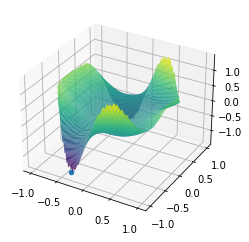
\includegraphics[width = 0.5\linewidth]{"./resources/random_min.png"}
	\caption{Минимум функции, найденный с помощью алгоритма случайного 
     поиска: \( x_{min} = -0.360171, y_{min} = 0.146528, f_{min} = -1.288383. \)}
    \label{fig:random_min}
\end{figure}

\anonsubsection{Метод имитации отжига}

Алгоритм основывается на имитации физического процесса, который происходит
 при кристаллизации вещества, в том числе при отжиге металлов. Предполагается,
 что атомы уже выстроились в кристалличекую решётку, но ещё допустимы переходы
 отдельных атомов из одной ячейки в другую. Предполагается, что процесс
 протекает при постепенно понижающейся температуре. Переход атома из одной 
 ячейки в другую происходит с некоторой вероятностью, причём вероятность 
 понижается с понижением температуры. Устойчивая кристаллическая решётка 
 соответствует минимуму энергии атомов, поэтому атом либо переходит в 
 состояние с меньшим уровнем энергии, либо остаётся на месте.

При помощи моделирования такого процесса ищется такая точка или множество 
 точек, на котором достигается минимум некоторой числовой функции 
 \( F(\overline{x}) \), где \( \overline{x}=(x_{1}, \dots,x_{m}) \in X \).
 Решение ищется последовательным вычислением точек \( \overline{x_0}, 
 \overline{x_1}, \dots, \) пространства \( X \); каждая точка, начиная с
 \( \overline{x_{1}} \), "<претендует"> на то, чтобы лучше предыдущих
 приближать решение. Алгоритм принимает точку \( \overline{x_{0}} \) как 
 исходные данные. На каждом шаге алгоритм (который описан ниже) вычисляет 
 новую точку и понижает значение величины (изначально положительной), 
 понимаемой как "<температура">. Алгоритм останавливается по достижении 
 точки, которая оказывается при температуре ноль.

Точка \( \overline{x_{i+1}} \) по алгоритму получается на основе текущей 
 точки \( \overline{x_{i}} \) следующим образом. К точке \( \overline{x_i}
 \) применяется оператор \( A \), который случайным образом модифицирует 
 соответствующую точку, в результате чего получается новая точка 
 \( \overline{x^*} \). Точка \( \overline{x^*} \) становится точкой 
 \( \overline{x_{i+1}} \) с вероятностью \( P \left( \overline{x^*}, 
 \overline{x_{i+1}} \right) \), которая вычисляется в соответствии с 
 распределением Гиббса:
\[
 P \left( \overline{x^*} \to \overline{x_{i+1}} | \overline{x_{i}} \right) 
 = \begin{cases} 
    1, & F( \overline{x^{*}} ) -F( \overline{x_{i}}) < 0,\\
    \exp \left( -\dfrac{F(\overline{x^{*}}) - F(\overline{x_{i}})}{T_i}
    \right), & F(\overline{x^{*}}) - F(\overline{x_{i}}) \geq 0.
 \end{cases}
\]

Здесь \( T_i>0 \)~---~элементы произвольной убывающей, сходящейся к нулю
 положительной последовательности, которая задаёт аналог падающей 
 температуры в кристалле. Скорость убывания и закон убывания могут быть 
 заданы по желанию создателя алгоритма.

Алгоритм имитации отжига похож на градиентный спуск, но за счёт случайности
 выбора промежуточной точки должен попадать в локальные минимумы реже, чем 
 градиентный спуск. Алгоритм имитации отжига не гарантирует нахождения 
 минимума функции, однако при правильной политике генерации случайной 
 точки в пространстве \( X \), как правило, происходит улучшение начального 
 приближения.

На Рис.\eqref{fig:sim_annealing} показан результат работы алгоритма, 
 включая промежуточные точки, в которых он оказывается.

\begin{figure}[ht]
	\centering
	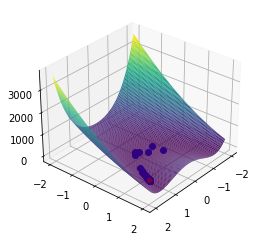
\includegraphics[width = 0.5\linewidth]{"./resources/sim_annealing.png"}
	\caption{Минимум функции, найденный с помощью алгоритма имитации отжига:
     \( x_{min} = 1.14533279, y_{min} = 1.31234433, f_{min} = 0.02115266.\)}
    \label{fig:sim_annealing}
\end{figure}

\anonsubsection{Оценка точности вычислений}
Пусть $x = (x_1, x_2)$ --- фактическая точка минимума, $\hat{x} = 
 (\hat{x}_1, \hat{x}_2)$ --- точка минимума, полученная методом случайного 
 поиска. Оценим $|x - \hat{x}|$.
Рассмотрим график исследуемой функции.

Исследуемая функция чётная по $x_1, x_2$, имеет несколько точек минимума, 
 которые не являются граничными. Тогда
\begin{equation*}
    |x - \hat{x}| \leq \varepsilon = \sqrt{\frac{p}{n}}.
\end{equation*}
Оценим $|f(x) - f(\hat{x})|$ через $|x - \hat{x}|$.\\
Поскольку $f$ --- непрерывна, то $f$ --- липшицева, следовательно:
\begin{equation*}
|f(a) - f(b)| \leq ||\nabla f||_\infty |a - b| = \underset{a, b\in A}{\esssup}
 |\nabla f| |a - b| = \max_{a, b \in A}|\nabla f| |a - b|, \forall a, b 
 \in A.
\end{equation*}
Оценим $\max\limits_{x_1, x_2 \in A} |\nabla f|$.\\
\begin{equation*}
\left|\frac{\partial f}{\partial x_1}\right| = \left|3x_1^2\sin(\frac{1}
 {x_1}) - x_1\cos(\frac{1}{x_1})+10x_2^4\cos(\frac{1}{x_2}) \right| \leq 
 3x_1^2+|x_1| +10x_2^4 \leq \sqrt{10} + 10,
\end{equation*}
\begin{equation*}
\left|\frac{\partial f}{\partial x_2}\right| = \left| 40x_1x_2^2 
 \cos(\frac{1}{x_2}) - 10x_1x_2^4 \cos(\frac{1}{x_2})\right| \leq 
 40|x_1|x_2^2 + 10|x_1|x_2^4 \leq 10\sqrt{17}.
\end{equation*}
Следовательно, $|\nabla f| = \sqrt{\left(\frac{\partial f}{\partial x_1} 
 \right)^2 + \left(\frac{\partial f}{\partial x_2}\right)} = 
 \sqrt{(\sqrt{10} + 10)^2+(10\sqrt{17})^2}\leq  34.26.$\\
Окончательная оценка точности вычислений:
\begin{equation*}
|f(x) - f(\hat{x})| \leq 34.26\sqrt{\frac{p}{n}}.
\end{equation*}
\anonsection{Задание 8}
\anonsubsection{Формулировка задания}

Применить метод Монте--Карло к решению первой краевой задачи для двумерного 
 уравнения Лапласа в единичном круге:
\begin{equation} \label{Dirichlet}
\left\lbrace
\begin{array}{lcr}
\Delta u=0,(x,y)\in D,\\
u|_{\delta D}=f(x,y),\\
u\in C^2(D),f\in C(\delta D),\\
D=\lbrace x,y:x^2+y^2\leqslant1\rbrace.
\end{array}
\right.
\end{equation}

Для функции \( f(x,y)=x^2-y^2 \) найти аналитическое решение и сравнить с 
 полученным по методу Монте--Карло.



\anonsubsection{Алгоритм решения}
Для приближенного решения задачи выберем на плоскости достаточно мелкую
квадратную сетку с шагом $h$. В таком случае, координатами узлов сетки 
 можно считать $x_j = jh, \ y_l = lh.$

\begin{definition}
	Будем называть узел сетки $(j, l)$ внутренним, если он и все четыре 
     соседних с ним узла
	$(j-1, l), \ (j + 1, l), \ (j, l - 1), \ (j, l + 1)$ принадлежат $D + 
     \delta D$, в противном случае узел $(j, l)$, принадлежащий $D + 
     \delta D$, будем называть граничным.
\end{definition} 

Во внутреннем узле \( (x_i,y_j) \) уравнение Лапласа \( u_{xx}+u_{yy}=0 \) 
 заменим разностным уравнением
\[
 \dfrac{u_{i + 1, j} - 2 u_{i, j} + u_{i - 1, j}}{h^2} + \dfrac{u_{i, j + 1} - 
  2 u_{i, j} + u_{i, j - 1}} {h^2} = 0,
\]
которое можно переписать в виде
\begin{equation} \label{internal}
u_{i,j}=\dfrac{1}{4}(u_{i-1,j}+u_{i+1,j}+u_{i,j-1}+u_{i,j+1}).
\end{equation}

В граничном узле положим
\begin{equation} \label{borders}
u_{i,j}=f_{i,j}.
\end{equation}

 

Представим себе частицу \( M \), которая совершает равномерное случайное 
 блуждание по узлам сетки. А именно, находясь во внутреннем узле 
 \( (x_i,y_j) \) сетки, эта частица за один переход с одинаковой 
 вероятностью \( 1/4 \) может переместиться в один из четырёх соседних 
 узлов, причём каждый такой единичный переход случаен и не зависит от 
 положения частицы и истории её передвижений. Будем считать, что блуждание 
 заканчивается, как только частица попадает в граничный узел. 

Пусть \( P(i,j,p,q) \)~---~вероятность того, что траектория частицы, 
 вышедшей из узла \( (x_i,y_j) \), закончится в граничном узле 
 \( (x_q,y_q) \). Так как блуждение точки неизбежно заканчивается на 
 границе в первой же точке выхода её на границу, то
\[
 \sum\limits_{(x_p,y_q)\in\delta D_h}P(i,j,p,q)=1,
\]
причём если \( (p',q'), (p,q)\in\delta D_h \), то
\[
P(p',q',p,q)=\begin{cases}
1,&(p'-p)^2+(q'-q)^2=0,\\
0,&(p'-p)^2+(q'-q)^2\ne0.
\end{cases}
\]

Составим сумму
\[
 v_{i,j}=\sum\limits_{(x_p,y_q)\in\delta D_h}P(i,j,p,q)f_{pq}.
\]

Если рассматривать функцию \( f(x,y) \) как случайную величину, принимающую 
 значения \( f_{pq} \) на границе \( \delta D_h \), то написанная выше 
 сумма представляет собой математическое ожидание функции \( f(x,y) \) на 
 границе \( \delta D_h \) для траекторий, начинающихся в узле \( (x_i,y_j) \). 
 Тогда в силу закона больших чисел можно аппроксимировать математическое 
 ожидание выборочным средним:
\[
 v_{i, j} \approx \dfrac{1}{N} \sum\limits_{k = 1}^{N} f \left( x_p^{(k)}, 
 y_q^{(k)} \right).
\]

Частица, начавшая своё случайное блуждание из внутреннего узла 
 \( (x_i,y_j) \), после первого шага с вероятностью, равной \( 1/4 \), 
 попадает в один из соседних четырёх узлов. Откуда по формуле полной 
 вероятности
\[
 v_{i, j} = \dfrac{1}{4} \sum\limits_{(x_p,y_q) \in\delta D_h} 
 (P(i - 1, j, p, q) + P(i + 1, j, p, q) + P(i, j - 1, p, q) + 
 P(i, j + 2, p, q))f_{p q} =
\]
\[
 = \dfrac{1}{4}(v_{i - 1, j} + v_{i + 1, j} + v_{i, j - 1} + v_{i,j + 1}).
\]
То есть во внутреннем узле \( (x_i, y_j) \)
\begin{equation} \label{internal_new}
    v_{i, j} = \dfrac{1}{4}(v_{i - 1, j} + v_{i + 1, j} + v_{i, j - 1} + 
     v_{i, j + 1}),
\end{equation}
в граничном узле
\begin{equation} \label{borders_new}
    v_{i, j} = f_{i, j}.
\end{equation}
 

По теореме о существовании решения внутренней задачи Дирихле решение 
 задачи ~ (\ref{Dirichlet}) существует. Найдем его для конкретной функции 
 \( f(x,y)=x^2-y^2 \). Будем искать его в виде \( u(x,y)=Ax^2+By^2+C \). 
 Подставив его в формулировку задачи, получим следующие условия на 
 коэффициенты:
\[
 \left\lbrace
 \begin{array}{rcl}
    A + B & = & 0,\\
    A - B & = & 2,\\
    B + C & = & -1;
\end{array}
\right.\quad\Longleftrightarrow\quad
\left\lbrace
\begin{array}{rcl}
A&=&1,\\
B&=&-1,\\
C&=&0;
\end{array}
\right.
\]

То есть мы получили, что функция \( u(x,y)=x^2-y^2 \) является решением 
 задачи~(\ref{Dirichlet}), причём решение единственно.

Согласно приведённым выше выкладкам, численное решение может быть найдено 
 по следующему алгоритму:

\begin{enumerate}
	\item Построим квадратную сетку на \( [-1,1]\times[-1,1] \) с шагом 
     \( \Delta \).
	
	\item Функцию во всех узлах, не принадлежащих кругу, положим равной 
     None.
	
	\item Все точки круга разделим на граничные и внутренние:
	
	\begin{itemize}
		\item В граничных точках положим \( u(x,y)=f(x,y) \).
		
		\item Значение в каждой внутренней точке получим следующим образом. 
         Попав во внутреннюю точку \( (x_i,y_j) \), проведём серию из 
         \( n \) случайных блужданий. Тогда
		\[
		u(x_i,y_j) = \dfrac{1}{n} \sum\limits_{k = 1}^{n} f \left( x_i^{(k)}, 
         y_i^{(k)} \right), 
		\]
		где \( \left( x_i^{(k)}, y_i^{(k)} \right) \)~---~граничная точка, в 
         которой завершилось \( k \)-е блуждание.
	\end{itemize}
\end{enumerate}

На Рис.\eqref{fig:boundary_solutions} изображены графики решения полученного по методу Монте-Карло
 и аналитического решения.

\begin{figure}[ht]
    \centering
    \begin{subfigure}[b]{0.45\textwidth}
        \centering
        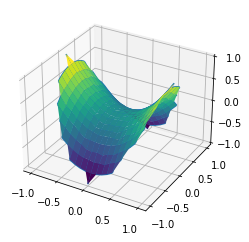
\includegraphics[width=\textwidth]{./resources/boundary_problem_emp.png}
        \caption{Решение по методу Монте-Карло.}
        \label{subfig:boundary_emp}
    \end{subfigure}
    \hfill
    \begin{subfigure}[b]{0.45\textwidth}
        \centering
        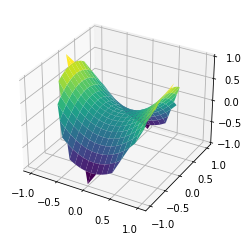
\includegraphics[width=\textwidth]{./resources/boundary_problem_an.png}
        \caption{Аналитическое решение: $ x^2 - y^2. $}
        \label{subfig:boundary_an}
    \end{subfigure}
    \caption{Решения задачи Дирихле.}
    \label{fig:boundary_solutions}
\end{figure}
\anonsection{Задание 9}
\anonsubsection{Формулировка задания}
Рассмотреть два вида процессов:
\begin{itemize}
	\item Винеровский процесс \( W(t), t\in[0,1], W(0) = 0 \).
	
	\item Процесс Орнштейна--Уленбека \( X(t), t\in[0,1], X(0) = X_0 \), 
     то есть стационарный марковский гауссовский процесс. Начальные 
     значения \( X_0 \) генеруются случайным образом так, чтобы полученный 
     процесс был стационарным.
	
\end{itemize}

Для данных гауссовских процессов
\begin{enumerate}
	\item Найти ковариационную функцию и переходные вероятности.
	
	\item Моделировать независимые траектории процесса с данными 
     переходными вероятностями методом добавления разбиения отрезка.
	
	\item Построить график траектории, не соединяя точки ломаной, с целью 
     получения визуально непрерывной линии.
\end{enumerate}

 
\anonsubsection{Винеровский процесс}

\begin{definition}
	Пусть дано вероятностное пространство \( (\Omega,\mathcal{F}, 
    \mathbb{P}) \). Параметризованное семейство \( \lbrace W_t\rbrace_{t \in 
     T} \) случайных величин
	\[
	 W_t(\cdot): \Omega \to \mathbb{R}, \quad t \in T,
	\]
	где \( T \subset[0, +\infty) \) интерпретируется как временной интервал, 
     называется случайным процессом.
\end{definition}
\begin{definition}
	Пусть дан случайный процесс \( \lbrace W_t \rbrace_{t\in T} \). Тогда 
     он называется гауссовским, если для любых \( t_0,t_1, \dots, t_n \in T \) 
     случайный вектор \( (W_{t_1}, W_{t_2}, \dots, W_{t_n}) \) имеет 
     многомерное нормальное распределение.
\end{definition}

Определим винеровский процесс как гауссовский процесс в отрезке 
 \( [0,1] \) со средним \( 0 \) и ковариационной функцией \( \text{cov} 
 \left(W(t_i), W(t_j) \right) = \min \left( t_i, t_j \right) \).

Основные свойства винеровского процесса:
\begin{itemize}
	\item $W_0=0$ почти наверное;
	\item $W_t$ является непрерывной функцией от $t$;
	\item Приращения функции $W(t)$ независимы и имеют нормальное 
     распределение со средним равным 0: $W_t - W_s \sim \mathcal{N} (0,1), 
     \quad s < t $.
\end{itemize}
Определим плотность $n$-мерного нормального распределения с невырожденной 
 ковариационной матрицей.
\begin{definition}
	Пусть $x$ --- $n$-мерный вектор и $ x \sim \mathcal{N}(m_x, R_x) $. 
     Тогда его плотность имеет вид
	\[
	 p(x) = \dfrac{1}{(2\pi)^{\frac{n}{2}}\sqrt{|R_x|}}e^ {-\frac{1}{2}
     (x-m_x)^T R_x^{-1}(x-m_x)},
	\]
	где $R_x$ --- ковариационная матрица.
\end{definition}
Смоделируем винеровский процесс методом деления отрезка $[0,1]$, в 
 отношении $\alpha$, исходя из следующих соображений:
\begin{enumerate}
	\item В начальный момент времени $W_{t_0}=0$, по определению;
	\item Генерируем $W_{t_1}=W_{t_1}-W_{t_0}\sim\mathcal{N}(0,1)$;
	\item Рассмотрим отрезок $[t_1,t_2]$, его внутреннюю точку $t = t_1 + 
     \alpha(t_2 - t_1)$ и условную плотность
	\begin{equation}\label{dens}
	    p_{W_t}(x \mid W_{t_1} = x_1, W_{t_2} = x_2) = \dfrac{p_{W_{t_1}, 
         W_t, W_{t_2}}(x_1, x, x_2)}{p_{W_{t_1}, W_{t_2}}(x_1, x_2)}. 
	\end{equation}
	 Обозначим векторы $ \bar{x} = (x_1, x, x_2)^T $ и $ \hat{x} = (x_1, 
     x_2)^T $ и рассмотрим плотности вероятностей этих векторов:
	$$
	\begin{aligned}
	    p_{W_{t_1}, W_t, W_{t_2}} & = \dfrac{1}{(2 \pi)^{\frac{3}{2}} 
         \sqrt{|R_1|}} e^{-\frac{1}{2} \bar{x}^T R_1^{-1} \bar{x}},\\
	    p_{W_{t_1}, W_{t_2}} &= \dfrac{1}{(2 \pi) \sqrt{|R_2|}} 
         e^{-\frac{1}{2}\hat{x}^T R_2^{-1} \hat{x}},
	\end{aligned}
	$$
	где $R_1,R_2$ --- соответствующие матрицы ковариаций. Так как 
     ковариационная функция имеет вид $k(s,t) = \min(s,t)$, то находим 
     выражения для $R_1$ и $R_2$:
	$$
	\begin{aligned}
	    & R_1 = \begin{pmatrix}
	        t_1 & t_1 & t_1 \\
	        t_1 & t & t \\
	        t_1 & t & t_2
	    \end{pmatrix} ,\\
	    & R_2 = \begin{pmatrix}
	        t_1 & t_1 \\
	        t_1 & t_2
	    \end{pmatrix}.
	\end{aligned}
	$$
	Вычислим определители и обратные матрицы для $R_1$ и $R_2$:
	\begin{gather*}
	|R_1|=t_1(t-t_1)(t_2-t), \\
	R_1^{-1}=\begin{pmatrix}
	\dfrac{t}{t_1(t-t_1)} & -\dfrac{1}{t-t_1} & 0 \\
	-\dfrac{1}{t-t_1} & \dfrac{t_2-t_1}{(t_2-t)(t-t_1} & -\dfrac{1}{t_2-t} \\
	0 & -\dfrac{1}{t_2-t} & \dfrac{1}{t_2-t}
	\end{pmatrix}, \\
	|R_2|=t_1(t_2-t_1), \\
	R_2^{-1}=\begin{pmatrix}
	\dfrac{t_2}{t_1(t_2-t_1)} & -\dfrac{1}{t_2-t_1} \\
	-\dfrac{1}{t_2-t_1} & \dfrac{1}{t_2-t_1}
	\end{pmatrix}.
	\end{gather*}
	В итоге получим:
	\begin{equation}\label{pW}
	    p_{W_t}(\,x \mid W_{t_1} = x_1, W_{t_2} = x_2\,) = \dfrac{1}{\sqrt{2 
         \pi \alpha (1 - \alpha)(t_2 - t_1)}} e^{-\dfrac{\left(x - ((1 - \alpha)
         x_1 + \alpha x_2) \right)^2}{2 \alpha(1 - \alpha)(t_2-t_1)}}. 
	\end{equation}
\end{enumerate}
Приведем итоговый алгоритм построения. 
\begin{enumerate}
	\item $t_0 = 0,\ t_1=1,\ W_{t_0}=0$, разыгрываем $W_{t_1} \sim 
     \mathcal{N}(0,1)$;
	\item Рекурсивно делим отрезки $[t_0,t_1],\ [t_0,t],\ [t,t_1]$ и т.~д. 
     в отношении $ \alpha $ к $ 1 - \alpha $ и разыгрываем случайные 
     величины $W_t$ с условной плотностью \eqref{pW} (то есть имеющие 
     нормальное распределение с математическим ожиданием $(1 - \alpha) 
     x_1 + \alpha x_2 $ и дисперсией $ \alpha(1 - \alpha)(t_2 - t_1)$) до 
     тех пор, пока не достигнем заданной точночти $t_{k + 1} - t_k < \epsilon$.
\end{enumerate}

\anonsubsection{Процесс Орнштейна--Уленбека}

\begin{definition}
	Случайный процесс \( \lbrace W_t\rbrace_{t\in T} \) называется 
     стационарным, если конечномерные распределения инвариантны 
     относительно сдвига времени.
\end{definition}

\begin{definition}
	Гауссовский процесс \( \lbrace W_t\rbrace_{t\in T} \) называется 
     процессом Орнштейна--Уленбека, если он является стационарным и 
     марковским.
\end{definition}

Из стационарности процесса Орнштейна--Уленбека следует, что
\[
\mathbb{E}W_t=a,\quad R(t,s)=R(|s-t|).
\]

Без ограничения общности положим \( a=0 \).

Обозначим \( \mathbb{D}W_t=\sigma^2 \), тогда \( R(t,s) \) представима в 
 виде \( R(t,s)=\sigma^2\rho(s,t) \), где \( \rho(s,t) \)~---~коэффициент 
 корреляции.

\begin{theorem}\footnote{Доказательство представлено в \cite{prob_feller}.}
	Для того чтобы последовательность \( W_1,\ldots,W_n \) нормально 
     распределённых случайных величин была марковской, необходимо и 
     достаточно, чтобы
	\[
	\rho_{j,k} = \rho_{j,i} \rho_{i,k} \ \forall i,j,k: j \leq i < k \leq n,
	\]
	где \( \rho_{i,j} \)~---~коэффициент корреляции случайных величин 
     \( W_i \) и \( W_j \).
\end{theorem}

В силу того, что процесс \( W_t \) является марковским, получаем, что
\begin{equation} \label{mark}
\rho(s,t)=\rho(s,\tau)\rho(\tau,t).
\end{equation}

Поскольку \( R(s,t)=R(|s-t|) \), то \( \rho(s,t)=\rho(s-t) \). Тогда, введя замену
\[
x=s-\tau,
\]
\[
y=\tau-t,
\]
преобразуем выражение~(\ref{mark}) к выражению
\[
\rho(x+y)=\rho(x)\rho(y).
\]

\begin{theorem}\footnote{Доказательство представлено в \cite{prob_feller}.}
	Пусть функция \( u(t) \) определена при \( t>0 \) и ограничена на 
     каждом конечном интервале. Если \( u(t) \) удовлетворяет соотношению 
     \( u(t+s)=u(t)u(s) \), то или \( u(t)\equiv0 \), или \( u(t) = 
     e^{-\lambda t} \), где \( \lambda \)~---~некоторая положительная 
     константа.
\end{theorem}

Если \( \rho(t) \equiv 0 \), то \( \text{cov}(W_t,W_s)=0 \), что 
 равносильно тому, что \( W_t \) независимы в совокупности (так как 
 процесс является гауссовским), поэтому поделирование процесса 
 Орнштейна--Уленбека заключается в моделировании случайных величин, 
 имеющих распределение \( N(a,\sigma^2) \).

Рассмотрим теперь случай \( \rho(s,t)=e^{-\lambda|s-t|} \), \( \lambda>0 \). 
 Ковариационная функция процесса Орнштейна--Уленбека имеет вид
\[
R(s,t)=\sigma^2e^{-\lambda|s-t|}.
\]

Найдём переходную плотность
\[
p_{W_t}(x_1|W_s=x_2)=\dfrac{p_{W_t,W_s}(x_1,x_2)}{p_{W_s}(x_2)}.
\]

Поскольку \( W_t \)~---~гауссовский процесс, то
\[
p_{W_t,W_s}(x_1,x_2)=\dfrac{1}{2\pi|C|^{\frac{1}{2}}}\exp\left\lbrace - 
 \dfrac{1}{2}(x,C^{-1}x)\right\rbrace,
\]
\[
p_{W_s}(x_2)=\dfrac{1}{\sqrt{2\pi}\sigma}\exp\left\lbrace - \dfrac{x_2^2}
 {2\sigma^2}\right\rbrace,
\]
где \( x=(x_1,x_2) \). Ковариационная матрица \( C \) имеет вид
\[
C=\begin{pmatrix}
\sigma^2&R(t,s)\\
R(t,s)&\sigma^2
\end{pmatrix}.
\]

Тогда
\[
|C|=\sigma^4-R^2(t,s), C^{-1}=\dfrac{1}{|C|}\begin{pmatrix}
\sigma^2&-R(t,s)\\
-R(t,s)&\sigma^2
\end{pmatrix}.
\]

Поэтому
\[
p_{W_t}(x_1|W_s=x_2)=\dfrac{1}{\left(2\pi\left(\sigma^2-\dfrac{R^2(t,s)}
 {\sigma^2}\right)\right)^{\frac{1}{2}}}\exp\left\lbrace-\dfrac{\left(x_1 - 
 \dfrac{R(t,s)}{\sigma^2}x_2\right)^2}{2\left(\sigma^2-\dfrac{R^2(t,s)}
 {\sigma^2}\right)}\right\rbrace,
\]
то есть
\[
F(W_t|W_s=x_2)\sim N\left(x_2e^{-\lambda|t-s|},\sigma^2\left(1-e^{-2 
 \lambda|t-s|}\right)\right).
\]

Так как рассматриваемый процесс является марковским, то, зная случайные 
 величины \( W_{t_1} \), \( W_{t_2} \), мы можем сгенерировать случайную 
 величину \( W_t \), где \( t_1<t<t_2 \). Будем моделировать \( W_t \) 
 аналогично моделированию винеровского процесса. Для упрощения положим 
 \( \alpha=1/2 \). Найдём условную плотность
\[
p_{W_{t}}(x|W_{t_1}=x_1,W_{t_2}=x_2)=\dfrac{p_{W_{t_1}W_tW_{t_2}}(x_1, x, 
 x_2)}{p_{W_{t_1},W_{t_2}}(x_1,x_2)},
\]
где \( t = (t_1 + t_2)/2 \). Поскольку процесс \( W_t \) является 
 гауссовским, то
\[
p_{W_{t_1}W_tW_{t_2}}(x_1,x,x_2) = \dfrac{1}{\left( 2 \pi \right)^{\frac{3}
 {2}} \left| R_1 \right|^{\frac{1}{2}}}\exp\left\lbrace-\dfrac{1}{2}(x_1, 
 x, x_2)^TR_1^{-1}(x_1,x,x_2)\right\rbrace,
\]
\[
p_{W_{t_1}W_{t_2}}(x_1,x_2)=\dfrac{1}{2\pi\left|R_2\right|^{\frac{1}{2}}} 
 \exp\left\lbrace-\dfrac{1}{2}(x_1,x_2)^TR_2(x_1,x_2)\right\rbrace,
\]
где
\[
R_1=\sigma^2\begin{pmatrix}
1&e^{-\lambda(t-t_1)}&e^{-\lambda(t_2-t_1)}\\
e^{-\lambda(t-t_1)}&1&e^{-\lambda(t_2-t)}\\
e^{-\lambda(t_2-t_1)}&e^{-\lambda(t_2-t)}&1
\end{pmatrix},\quad
R_2=\sigma^2\begin{pmatrix}
1&e^{-\lambda(t_2-t_1)}\\
e^{-\lambda(t_2-t_1)}&1
\end{pmatrix}.
\]

После ряда преобразований получим
\[
W_t\sim N\left((x_1+x_2)\dfrac{e^{-\frac{\lambda(t_2-t_1)}{2}}}{1 + 
 e^{-\lambda(t_2-t_1)}},\sigma^2\dfrac{1-e^{-\lambda(t_2-t_1)}}{1 + 
 e^{-\lambda(t_2-t_1)}}\right).
\]

В качестве \( W_0 \) и \( W_1 \) возьмём
\[
W_0\sim N(0,\sigma^2),W_1\sim N\left(x_0e^{-\lambda T}, \sigma^2\left(1 - 
 e^{-2\lambda T}\right)\right).
\]

\begin{figure}[ht]
    \centering
    \begin{subfigure}[b]{0.49\textwidth}
        \centering
        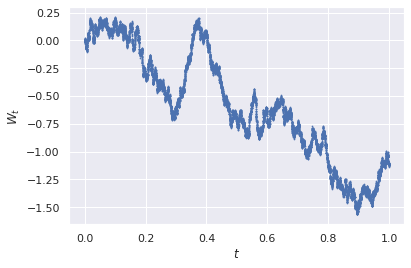
\includegraphics[width=\textwidth]{./resources/wiener_process.png}
        \caption{Винеровский процесс на отрезке $ [0, 1] $.}
        \label{subfig:wiener}
    \end{subfigure}
    \hfill
    \begin{subfigure}[b]{0.49\textwidth}
        \centering
        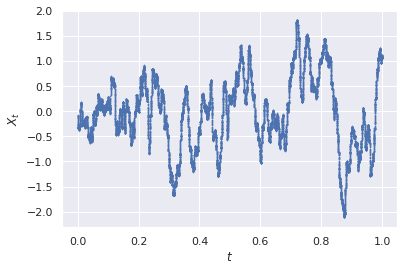
\includegraphics[width=\textwidth]{./resources/Orn_Uhl_process.png}
        \caption{Процесс Орнштейна-Уленбека на отрезке $ [0, 1] $.}
        \label{subfig:Orn_Uhl}
    \end{subfigure}
    \caption{Графики смоделированных процессов.}
    \label{fig:processes}
\end{figure}
\anonsection{Задание 10}
\anonsubsection{Формулировка задания}

Произвести фильтрацию одномерного процесса Орнштейна--Уленбека:
\begin{enumerate}
	\item Используя генератор белого шума, добавить случайную ошибку с 
     известной дисперсией к реализации процесса Орнштейна--Уленбека.
	
	\item При помощи одномерного фильтра Калмана оценить траекторию 
     процесса по зашумленному сигналу. Параметры процесса и белого шума 
     считать известными.
	
	\item Рассмотреть случай, когда шум
	
	\begin{itemize}
		\item Является гауссовским.
		
		\item Имеет распределение Коши.
		
	\end{itemize}
	
\end{enumerate}


\anonsubsection{Добавление случайной ошибки}

\begin{definition}
	Дискретным белым шумом называется последовательность \( \varepsilon_1, 
     \ dots, \varepsilon_n, \dots \) независимых одинаково распределённых 
     случайных величин.
\end{definition}

Рассмотрим соотношение 
\[
x_{k+1}=f(x_k)+\omega(k),
\]
где \( \omega(k) \)~---~случайная помеха, \( x_k \), \( \omega(k) \) 
 независимы, \( f(x_k)=\mathbb{E}(x_{k+1}|x_k) \). Пусть рассматривается 
 марковский процесс, тогда совместная плотность по всем моментам времени
\[
p(x_k,\ldots,x_0)=p(x_k|x_{k-1},\ldots,x_0)\cdot p(x_{k-1}|x_{k-2}, \dots, 
 x_0) \cdot \ldots \cdot p(x_1|x_0) \cdot p(x_0)=
\]
\[
=\lbrace\text{марковский процесс}\rbrace=p(x_k|x_{k-1})\cdot p(x_{k-1} 
| x_{k-2}) \cdot \ldots \cdot p(x_1|x_0)\cdot p(x_0).
\]
Обратим внимание, что в случае, когда шум имеет распределение Коши, 
 фильтрацию провести не получится. Это связанно с тем, что распределение 
 Коши не имеет математического ожидания.  Далее будем рассматривать случай, 
 когда шум является гауссовским (\( \omega(k) \) и \( x_k \) имеют 
 гауссовское распределение).


\anonsubsection{Фильтр Калмана}

Рассмотрим линейное стохастическое уравнение
\[
x_{k+1}=A_kx_k+\omega_k.
\]

Поскольку случайные величины гауссовские, то для их полного описания 
 достаточно знать их первые и вторые моменты.

Пусть имеется следующая система:
\begin{equation} \label{kalman_syst}
\left\lbrace
\begin{array}{rcl}
x_{k+1}&=&A_kx_k+w_k,\\
y_{k+1}&=&C_{k+1}x_{k+1}+v_{k+1},
\end{array}
\right.
\end{equation}
причём \( x_0, w_0,\ldots, w_{N-1},v_0,\ldots,v_{n-1} \) независимы в 
 совокупности. \( Y_{N-1}=(y_0,\ldots,y_{N-1})^T \)~---~все наблюдения, 
 а \( X_{N-1}=(x_0,\ldots,x_{N-1}) \)~---~исходный процесс, его надо найти. 
 Для этого воспользуемся так называемым фильтром Калмана, а точнее, его 
 схемой "<шагаем--мерим">, общий вид которой совпадает с 
 системой~(\ref{kalman_syst}). 

Обозначим \( \mathbb{E} x_0 = \overline{x}_0, \mathbb{D}x_0 = S, 
 \mathbb{E} w_k = \mathbb{E}v_k = 0, \mathbb{D} w_k = M_k, \mathbb{D}v_k = 
 N_k>0 \). Фильтр Калмана для схемы "<шагаем--мерим"> имеет вид:
\[
\left\lbrace
\begin{array}{rcl}
\hat{x}_{k+1|k}&=&A_k\hat{x}_{k|k},\\
\hat{x}_{k+1|k+1}&=&\hat{x}_{k+1|k}+R_{k+1|k}C^T_{k+1}(C_{k+1}R_{k+1|k} 
 C^T_{k+1}+N_{k+1})^{-1}(y_{k+1}-C_{k+1}\hat{x}_{k+1|k}),\\
R_{k+1|k}&=&A_kR_{k|k}A_k^T+M_k,\\
R_{k+1|k+1}&=&R_{k+1|k}-R_{k+1|k}C^T_{k+1}(C_{k+1}R_{k+1|k}C_{k+1}^T+
 N_{k+1})^{-1}C_{k+1}R_{k+1|k},\\
\hat{x}_{0|0}&=&\overline{x}_0,\\
R_{0|0}&=&S.
\end{array}
\right.
\]

В нашей задаче \( x_{k} \)~---~процесс Орнштейна--Уленбека с параметрами 
 \( \sigma_W \) и \( \lambda \), \( y_{k+1}=x_{k+1}+v_{k+1} \), где 
 \( v \)~---~белый шум. Пусть \( \sigma_n^2 \)~---~его дисперсия. Тогда 
 получаем, что \( N_k=\sigma_n^2 \), а \( C_k=1 \). Осталось найти 
 \( A_k \) и \( M_k \). Будем считать, что \( t_{i+1}-t_i=\Delta t \) 
 независимо от \( i \). Так как мы рассматриваем одномерный процесс 
 Орнштейна--Уленбека, то \( A_k,C_k \) являются скалярами, и от их 
 транспонирования ничего не меняется. Обозначим \( \mathbb{D}x_k=V_k \). 
 С одной стороны, имеем
\[
\mathbb{D}x_{k+1}=A_k^2\mathbb{D}x_{k}+\mathbb{D}w_k=A_k^2V_k+M_k,
\]
\[
\text{cov}(x_{k+1},x_k)=\mathbb{E}(x_{k+1}x_k)-\mathbb{E}x_{k+1}\mathbb{E}
 x_k=\mathbb{E}(A_kx_k^2+w_{k+1}x_{k})-A_k(\mathbb{E}x_k)^2=
\]
\[
=\lbrace\mathbb{E}w_{k+1}=0,w_{k+1}\text{ и }x_k\text{ независимы}\rbrace = 
 A_k\left(\mathbb{E}x_k^2-(\mathbb{E}x_k)^2\right)=A_k\mathbb{D}x_k=A_kV_k.
\]

С другой стороны, так как ковариационная функция процесса Орнштейна--Уленбека 
 имеет вид \( R(t,s)=\sigma^2_We^{-\lambda|t-s|} \), то получим следующую 
 систему уравнений:
\[
\left\lbrace
\begin{array}{lcr}
A_k^2V_k+M_k=\sigma_W^2,\\
A_kV_k=\sigma_W^2e^{-\lambda\Delta t},\\
V_k=\sigma_W^2.
\end{array}
\right.
\]

Получаем, что \( V_k=\sigma_W^2 \), \( A_k=e^{-\lambda\Delta t} \), а 
 \( M_k=\sigma_W^2(1-e^{-2\lambda\Delta t}) \). Обратим внимание, что 
 когда мы в предыдущем задании вводили процесс Орнштейна--Уленбека, то 
 считали, что \( \mathbb{D}x_k=\sigma_W^2 \), что согласуется с тем, что 
 мы получили.

Тогда фильтр Калмана для нашей задачи имеет вид:

\[
\left\lbrace
\begin{array}{rcl}
\hat{x}_{k+1|k}&=&e^{-\lambda\Delta t}\hat{x}_{k|k},\\
\hat{x}_{k+1|k+1}&=&\hat{x}_{k+1|k}+R_{k+1|k}(R_{k+1|k}+\sigma_n^2)^{-1}
 (y_{k+1}-\hat{x}_{k+1|k}),\\
R_{k+1|k}&=&e^{-2\lambda\Delta t}R_{k|k}+\sigma^2_W(1-e^{-2\lambda\Delta t}),\\
R_{k+1|k+1}&=&R_{k+1|k}-R_{k+1|k}(R_{k+1|k}+\sigma^2_n)^{-1}R_{k+1|k},\\
\hat{x}_{0|0}&=&0,\\
R_{0|0}&=&\sigma^2_W.
\end{array}
\right.
\]

Обозначив \( h=R_{k+1|k}(R_{k+1|k}+\sigma^2_n)^{-1} \), получим итоговую 
 систему:
\[
\left\lbrace
\begin{array}{rcl}
\hat{x}_{k+1|k}&=&e^{-\lambda\Delta t}\hat{x}_{k|k},\\
R_{k+1|k}&=&e^{-2\lambda\Delta t}R_{k|k}+\sigma^2_W(1-e^{-2\lambda\Delta t}),\\
h&=&R_{k+1|k}(R_{k+1|k}+\sigma^2_n)^{-1},\\
\hat{x}_{k+1|k+1}&=&(1-h)\hat{x}_{k+1|k}+hy_{k+1},\\
R_{k+1|k+1}&=&(1-h)R_{k+1|k},\\
\hat{x}_{0|0}&=&0,\\
R_{0|0}&=&\sigma^2_W.
\end{array}
\right.
\]

На Рис.\eqref{fig:filter} изображен резултат применения фильтра Калмана к
 зашумленному процессу Орнштейна-Уленбека в случае Гауссовского шума и шума 
 Коши. Видно, что во втором случае результат фильтрации неудовлетворителен.

\begin{figure}[ht]
    \centering
    \begin{subfigure}[b]{0.49\textwidth}
        \centering
        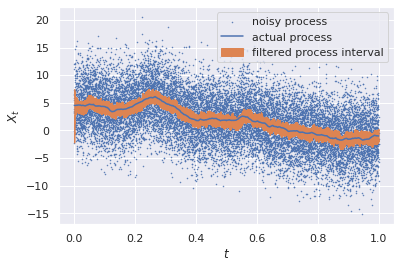
\includegraphics[width=\textwidth]{./resources/Gauss_filter.png}
        \caption{Фильтрация процесса с гауссовским шумом.}
        \label{subfig:Gauss_filter}
    \end{subfigure}
    \hfill
    \begin{subfigure}[b]{0.49\textwidth}
        \centering
        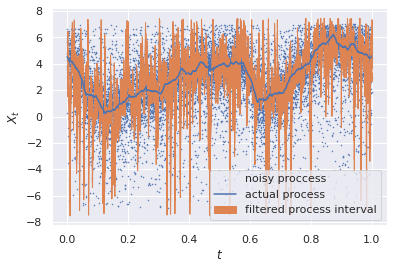
\includegraphics[width=\textwidth]{./resources/Cauchy_filter.png}
        \caption{Фильтрация процесса с шумом распределнным по Коши.}
        \label{subfig:Cauchy_filter}
    \end{subfigure}
    \caption{Фильтрация процесса Орнштейна-Уленбека.}
    \label{fig:filter}
\end{figure}
\anonsection{Задание 11}
\anonsubsection{Формулировка задания}
Построить двумерное пуассоновское поле, отвечающее сложному 
 пуассоновскому процессу:

\begin{enumerate}
	\item Первая интерпретация: система массового обслуживания. При этом 
     первая координата поля~---~время поступления заявки в СМО 
     (равномерное распределение), вторая~---~время её обслуживания 
     (распределение \( \chi^2 \) с \( 10 \)-ю степенями свободы).
	
	\item Вторая интерпретация: система массового обслуживания с 
     циклической интенсивностью \( \lambda(t)=\lambda_0(1+\cos(t)) \) и 
     единичными скачками. Свести данную задачу моделирования 
     неоднородного пуассоновского процесса при помощи метода Льюиса и 
     Шедлера к моделированию двумерного пуассоновского поля, где первая 
     координата имеет равномерное распределение, а вторая~---~распределение 
     Бернулли.
	
	\item Третья интерпретация: работа страховой компании. Первая 
     координата~---~момент наступления страхового случая (равномерное 
     распределение), вторая координата~---~величина ущерба (распределение 
     Парето). Поступление капитала по времени линейно со скоростью 
     \( c>0 \), начальный капитал \( W>0 \).
	
	\item Для каждой системы рассмотреть всевозможные случаи поведения 
     системы в зависимости от значения параметров.
	
\end{enumerate}




\anonsubsection{Первая интерпретация: система массового обслуживания}
Пусть $\lambda$ --- интенсивность пуассоновского поля. Времена 
 поступления заявок генерируются так, что $\Delta t_i = t_i - t_{i - 1} 
 \sim Exp(\lambda)$.
 Время обслуживания каждой заявки $s_i$ независимы и генерируются как 
 случайные величины с распределением $\chi^2(10)$.\\
Поскольку все заявки обрабатываются последовательно, время окончания 
 обработки заявки, поступившей в момент времени $t_i$ можно найти 
 следующим образом:
\begin{itemize}
	\item если к моменту поступления заявки предыдущая заявка уже 
     обработана, то нужно к времени поступления текущей заявки прибавить 
     время ее обработки;
	\begin{center}
		$Q_i = t_i + s_i.$
	\end{center}
	\item если предыдущая заявка еще не обработана, то нужно прибавить к 
     времени конца обработки предыдущей заявки время обработки текущей.
\begin{center}
		$Q_i = Q_{i-1} + s_i.$
\end{center}

\end{itemize}
Обобщая вышесказанное, имеем:
\begin{center}
		$Q_i = t_i + \max(0, Q_{i - 1} - t_i) + s_i.$
\end{center}

Для каждой заявки будем считать количество людей в очереди.

\begin{itemize}
	\item если во время поступления $i$-й заявки очереди не было, то 
     положим $n_i = 0$.

	\item если предыдущая заявка еще не обработана, то 
	
	\begin{center}
		$n_i \neq Q_k : k < i$ и $Q_k > t_i$
	\end{center}
т. е. количество еще не выполненных к моменту времени $t_i$ заявок.
\end{itemize}

Поскольку время обработки одной заявки в среднем равно 10, а средний 
 интервал между поступлениями заявок равен $\mathbb{E}\Delta_i = 
 \frac{1}{\lambda}$, то при $\lambda < 0.1$ очереди практически не 
 будет, а при $\lambda > 0.1$ очередь будет неограниченно расти. Этот
 эффект продемонстрирован на Рис.\eqref{fig:queuing}.

\begin{figure}[ht]
    \centering
    \begin{subfigure}[b]{0.49\textwidth}
        \centering
        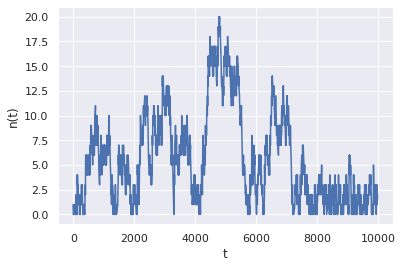
\includegraphics[width=\textwidth]{./resources/queuing_0.09.png}
        \caption{Моделирование очереди при $ \lambda = 0.09 $. Система 
         справляется.}
        \label{subfig:queuing_0.09}
    \end{subfigure}
    \hfill
    \begin{subfigure}[b]{0.49\textwidth}
        \centering
        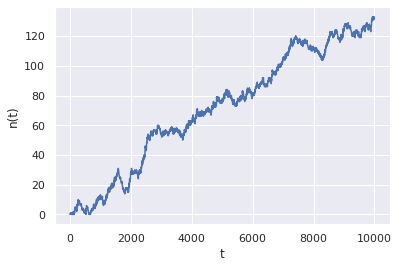
\includegraphics[width=\textwidth]{./resources/queuing_0.11.png}
        \caption{Моделирование очереди при $ \lambda = 0.11 $. Очередь 
         растет.}
        \label{subfig:queuing_0.11}
    \end{subfigure}
    \caption{Моделирование очереди при разных показателях интенсивности.}
    \label{fig:queuing}
\end{figure}

\anonsubsection{Вторая интерпретация: система массового обслуживания с 
циклической интенсивностью  и единичными скачками}


Пусть \( T_1,\ldots,T_n,\ldots \)~---~времена наступления некоторых 
 событий, а \( N(t_1,t_2) \)~---~количество событий, произошедших в 
 промежуток \( [t_1,t_2] \). Заметим, что \( T_{n+1}-T_n \) имеет 
 функцию распределения \( F(x)=1-e^{-(\Lambda(t+x)-\Lambda(t))}, x 
 \geq 0 \), где 


\[
 \Lambda(t)=\int\limits_0^t\lambda(u)du=\lambda(t+\sin t).
\]
неограниченно возрастает с ростом \( t \). 

\( T_{n+1} \) распределено как \( T_n+F^{-1}(U) \), где \( U \) 
 равномерно распределена на \( [0,1] \). Заметим, что если записать 
 \( U \) как \( 1-e^{-E} \), где \( E \)~---~экспоненциальная случайная 
 величина с параметром \( \lambda_E=1 \), то \( T_{n+1} \) распределена 
 как \( \Lambda^{-1}(E+\Lambda(T_n)) \).

Будем искать обратную функцию \( \Lambda^{-1}(y) \) численно, так как 
 аналитически это не представляется возможным ( \( \Lambda'(t) = 
 \lambda_0(1+\cos(t)) \)) почти всюду положительна, то есть функция 
 возрастает). Такой метод моделирования неоднородного процесса Пуассона 
 называется методом Льюиса--Шедлера.

Чтобы не искать обратную функцию, можно воспользоваться следующей 
 модификацией метода Льюиса--Шедлера. Пусть имеется переменная \( t \), 
 в которой хранится текущее время (но не обязательно событие произошло 
 строго в это время). 

\begin{itemize}
	\item На каждом шаге генерируем случайную величину \( \xi \sim 
     \Exp(2\lambda_0) \).
	\item Прибавляем к переменной \( t \) величину \( \xi \) и генерируем 
     случайную величину \( \eta=\Bern((1+\cos t)/2) \).
	\begin{itemize}
			\item если она приняла значение \( 1 \), то полагаем 
             \( T_{i+1}=t \) и \( i=i+1 \)
			\item иначе ничего не делаем и повторяем процесс заново
	\end{itemize}
\end{itemize}

На Рис.\eqref{fig:queuing_cycling} изображена смоделированная система с 
 циклической интенсивностью. Промежуткам роста длины очереди соответсвуют
 промежутки возрастания интенсивности.
\begin{figure}[ht]
	\centering
	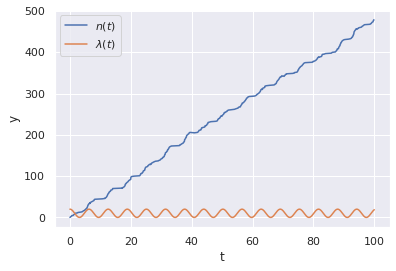
\includegraphics[width = 0.7\linewidth]{"./resources/queuing_cycling.png"}
	\caption{Система массового обслуживания с циклической интенсивностью.}
    \label{fig:queuing_cycling}
\end{figure}

\anonsubsection{Третья интерпретация: работа страховой компании.}
\begin{definition}
	Случайная величина $X$ имеет распределение Парето с параметрами 
     $x_m$ и $k$, если ее функция распределения имеет вид:
	\begin{equation*}
	F_X(x) = 1 - \left(\frac{x_m}{x}\right)^k.
	\end{equation*}
\end{definition}
Для моделирования случайной величины, имеющей распределение Парето, 
 снова воспользуемся методом обратной функции.\\
Обратная функция для данной функции распределения имеет вид:
\begin{equation}
F_X^{-1}(x) = \frac{x_m}{(1 - x)^{\frac{1}{k}}}.
\end{equation}

Сгенерируем времена наступления страховых случаев на временном интервале 
 \( [0,T] \):
\[
0 \leq t_1 \leq t_2 \leq \ldots \leq t_n \leq T,
\]
причём \( t_i-t_{i-1} \sim \Exp(\lambda) \), \( \lambda>0 \)~---~интенсивность 
 потока страховых случаев.

Величину ущерба \( s_i \) страхового случая в момент времени \( t \) 
 будем генерировать с помощью распределения Парето с параметрами 
 \( x_m \) и \( k \). Случайную величину, распределённую по Парето, 
 будем генерировать, воспользовавшись методом обратных функций:
\[
F_{\xi}^{-1}(y)=\dfrac{x_m}{\left(1-x\right)^{\frac{1}{k}}}.
\]

Учтем, что если \( Y\sim U[0,1] \), то и \( (1-Y)\sim U[0,1] \). Тогда 
 случайная величина
\[
X=x_mY^{-\frac{1}{k}},\quad Y\sim U[0,1]
\]
имеет распределение Парето с параметрами \( x_m \) и \( k \).

Величина капитала компании в момент времени \( t \) выражается как
\[
W_t=W_0+ct-s(t),
\]
где \( s(t) \)~---~сумма величин ущерба страховых случаев, произошедших 
 в моменты времени \( t_i \) такие, что \( t_i\leqslant t \). Время 
 разорения~---~случайная величина, задаваемая следующим условием:
\[
T=\min\lbrace t>0|W_t<0\rbrace.
\]

Выведем зависимость функции \( W(t) \) от параметров \( \lambda \), 
 \( x_m \), \( k \), \( W_0 \), \( c \). Будем считать, что \( k>1 \). 
 Тогда
\[
\mathbb{E}W'(t)=c-\mathbb{E}'s(t)=c-\left(\mathbb{E}\left[\sum\limits_{t_i<t}
 s_i\right]\right)'=c-\left(\dfrac{t}{\frac{1}{\lambda}}\mathbb{E}[s_i]
 \right)'=c-\dfrac{\lambda kx_m}{k-1}.
\]

Таким образом,
\begin{itemize}
	\item при \( c(k-1)>\lambda k x_m \) капитал растёт
	\item при \( c(k-1)=\lambda k x_m \) система находится в положении 
     равновесия
	\item при \( c(k-1)<\lambda k x_m \) капитал уменьшается
\end{itemize}

На Рис.\eqref{fig:ins_comp} изображено уменьшение, баланс и рост капитала
 компании в зависимости от параметров.

\begin{figure}[ht]
    \centering
    \begin{subfigure}[b]{0.49\textwidth}
        \centering
        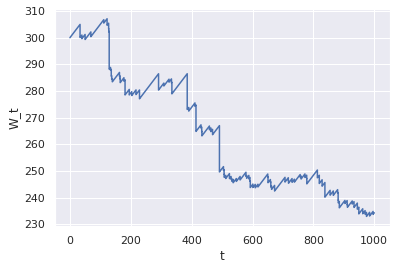
\includegraphics[width=\textwidth]{./resources/ins_comp_decreasing.png}
        \caption{Уменьшение капитала: $\lambda = 0.1, x_m = 1, k = 2, c = 0.15. $}
        \label{subfig:ins_comp_decreasing}
    \end{subfigure}
    \hfill
    \begin{subfigure}[b]{0.49\textwidth}
        \centering
        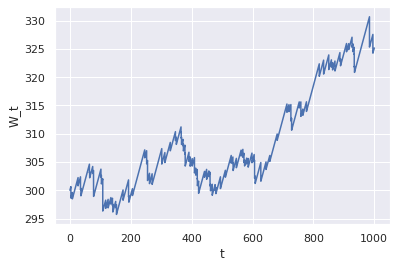
\includegraphics[width=\textwidth]{./resources/ins_comp_balancing.png}
        \caption{Баланс капитала: $\lambda = 0.1, x_m = 1, k = 2, c = 0.2. $}
        \label{subfig:ins_comp_balancing}
    \end{subfigure}
    \hfill
    \begin{subfigure}[b]{0.49\textwidth}
        \centering
        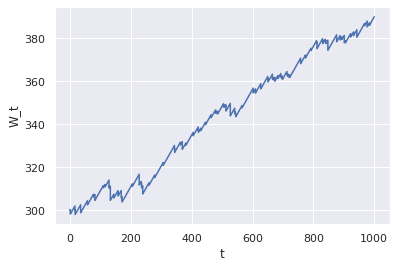
\includegraphics[width=\textwidth]{./resources/ins_comp_increasing.png}
        \caption{Увеличение капитала: $\lambda = 0.1, x_m = 1, k = 2, c = 0.25. $}
        \label{subfig:ins_comp_increasing}
    \end{subfigure}
    \caption{Моделирование капитала страховой компании.}
    \label{fig:ins_comp}
\end{figure}

\begin{thebibliography}{0}
	\addcontentsline{toc}{section}{Список литературы}
	\bibitem{lagutin_stat} Лагутин~М.\,Б.
	\emph{Наглядная метематическая статистика}, Бином. М.: 2009.
	
	\bibitem{model_randoms} Кропачёва~Н.\,Ю., Тихомиров~А.\,С.
	\emph{Моделирование случайных величин}, НовГУ им. Ярослава
     Мудрого. Великий Новгород: 2004.

	\bibitem{shir_prob} Ширяев~А.\,Н.
	\emph{Вероятность}, МЦНМО. М.: 2007.
\end{thebibliography}
\end{document}